\documentclass[]{book}
\usepackage{lmodern}
\usepackage{amssymb,amsmath}
\usepackage{ifxetex,ifluatex}
\usepackage{fixltx2e} % provides \textsubscript
\ifnum 0\ifxetex 1\fi\ifluatex 1\fi=0 % if pdftex
  \usepackage[T1]{fontenc}
  \usepackage[utf8]{inputenc}
\else % if luatex or xelatex
  \ifxetex
    \usepackage{mathspec}
  \else
    \usepackage{fontspec}
  \fi
  \defaultfontfeatures{Ligatures=TeX,Scale=MatchLowercase}
\fi
% use upquote if available, for straight quotes in verbatim environments
\IfFileExists{upquote.sty}{\usepackage{upquote}}{}
% use microtype if available
\IfFileExists{microtype.sty}{%
\usepackage{microtype}
\UseMicrotypeSet[protrusion]{basicmath} % disable protrusion for tt fonts
}{}
\usepackage[margin=1in]{geometry}
\usepackage{hyperref}
\hypersetup{unicode=true,
            pdftitle={Curso de R para Meteorologia IAG/USP},
            pdfauthor={Sergio Ibarra-Espinosa, Amanda Rehbein, Daniel Schuch, Camila Lopes, Isabela Siqueira, e possivelmente outros (você está convidado para colaborar)},
            pdfborder={0 0 0},
            breaklinks=true}
\urlstyle{same}  % don't use monospace font for urls
\usepackage{natbib}
\bibliographystyle{apalike}
\usepackage{color}
\usepackage{fancyvrb}
\newcommand{\VerbBar}{|}
\newcommand{\VERB}{\Verb[commandchars=\\\{\}]}
\DefineVerbatimEnvironment{Highlighting}{Verbatim}{commandchars=\\\{\}}
% Add ',fontsize=\small' for more characters per line
\usepackage{framed}
\definecolor{shadecolor}{RGB}{248,248,248}
\newenvironment{Shaded}{\begin{snugshade}}{\end{snugshade}}
\newcommand{\KeywordTok}[1]{\textcolor[rgb]{0.13,0.29,0.53}{\textbf{#1}}}
\newcommand{\DataTypeTok}[1]{\textcolor[rgb]{0.13,0.29,0.53}{#1}}
\newcommand{\DecValTok}[1]{\textcolor[rgb]{0.00,0.00,0.81}{#1}}
\newcommand{\BaseNTok}[1]{\textcolor[rgb]{0.00,0.00,0.81}{#1}}
\newcommand{\FloatTok}[1]{\textcolor[rgb]{0.00,0.00,0.81}{#1}}
\newcommand{\ConstantTok}[1]{\textcolor[rgb]{0.00,0.00,0.00}{#1}}
\newcommand{\CharTok}[1]{\textcolor[rgb]{0.31,0.60,0.02}{#1}}
\newcommand{\SpecialCharTok}[1]{\textcolor[rgb]{0.00,0.00,0.00}{#1}}
\newcommand{\StringTok}[1]{\textcolor[rgb]{0.31,0.60,0.02}{#1}}
\newcommand{\VerbatimStringTok}[1]{\textcolor[rgb]{0.31,0.60,0.02}{#1}}
\newcommand{\SpecialStringTok}[1]{\textcolor[rgb]{0.31,0.60,0.02}{#1}}
\newcommand{\ImportTok}[1]{#1}
\newcommand{\CommentTok}[1]{\textcolor[rgb]{0.56,0.35,0.01}{\textit{#1}}}
\newcommand{\DocumentationTok}[1]{\textcolor[rgb]{0.56,0.35,0.01}{\textbf{\textit{#1}}}}
\newcommand{\AnnotationTok}[1]{\textcolor[rgb]{0.56,0.35,0.01}{\textbf{\textit{#1}}}}
\newcommand{\CommentVarTok}[1]{\textcolor[rgb]{0.56,0.35,0.01}{\textbf{\textit{#1}}}}
\newcommand{\OtherTok}[1]{\textcolor[rgb]{0.56,0.35,0.01}{#1}}
\newcommand{\FunctionTok}[1]{\textcolor[rgb]{0.00,0.00,0.00}{#1}}
\newcommand{\VariableTok}[1]{\textcolor[rgb]{0.00,0.00,0.00}{#1}}
\newcommand{\ControlFlowTok}[1]{\textcolor[rgb]{0.13,0.29,0.53}{\textbf{#1}}}
\newcommand{\OperatorTok}[1]{\textcolor[rgb]{0.81,0.36,0.00}{\textbf{#1}}}
\newcommand{\BuiltInTok}[1]{#1}
\newcommand{\ExtensionTok}[1]{#1}
\newcommand{\PreprocessorTok}[1]{\textcolor[rgb]{0.56,0.35,0.01}{\textit{#1}}}
\newcommand{\AttributeTok}[1]{\textcolor[rgb]{0.77,0.63,0.00}{#1}}
\newcommand{\RegionMarkerTok}[1]{#1}
\newcommand{\InformationTok}[1]{\textcolor[rgb]{0.56,0.35,0.01}{\textbf{\textit{#1}}}}
\newcommand{\WarningTok}[1]{\textcolor[rgb]{0.56,0.35,0.01}{\textbf{\textit{#1}}}}
\newcommand{\AlertTok}[1]{\textcolor[rgb]{0.94,0.16,0.16}{#1}}
\newcommand{\ErrorTok}[1]{\textcolor[rgb]{0.64,0.00,0.00}{\textbf{#1}}}
\newcommand{\NormalTok}[1]{#1}
\usepackage{longtable,booktabs}
\usepackage{graphicx,grffile}
\makeatletter
\def\maxwidth{\ifdim\Gin@nat@width>\linewidth\linewidth\else\Gin@nat@width\fi}
\def\maxheight{\ifdim\Gin@nat@height>\textheight\textheight\else\Gin@nat@height\fi}
\makeatother
% Scale images if necessary, so that they will not overflow the page
% margins by default, and it is still possible to overwrite the defaults
% using explicit options in \includegraphics[width, height, ...]{}
\setkeys{Gin}{width=\maxwidth,height=\maxheight,keepaspectratio}
\IfFileExists{parskip.sty}{%
\usepackage{parskip}
}{% else
\setlength{\parindent}{0pt}
\setlength{\parskip}{6pt plus 2pt minus 1pt}
}
\setlength{\emergencystretch}{3em}  % prevent overfull lines
\providecommand{\tightlist}{%
  \setlength{\itemsep}{0pt}\setlength{\parskip}{0pt}}
\setcounter{secnumdepth}{5}
% Redefines (sub)paragraphs to behave more like sections
\ifx\paragraph\undefined\else
\let\oldparagraph\paragraph
\renewcommand{\paragraph}[1]{\oldparagraph{#1}\mbox{}}
\fi
\ifx\subparagraph\undefined\else
\let\oldsubparagraph\subparagraph
\renewcommand{\subparagraph}[1]{\oldsubparagraph{#1}\mbox{}}
\fi

%%% Use protect on footnotes to avoid problems with footnotes in titles
\let\rmarkdownfootnote\footnote%
\def\footnote{\protect\rmarkdownfootnote}

%%% Change title format to be more compact
\usepackage{titling}

% Create subtitle command for use in maketitle
\newcommand{\subtitle}[1]{
  \posttitle{
    \begin{center}\large#1\end{center}
    }
}

\setlength{\droptitle}{-2em}
  \title{Curso de R para Meteorologia IAG/USP}
  \pretitle{\vspace{\droptitle}\centering\huge}
  \posttitle{\par}
  \author{Sergio Ibarra-Espinosa, Amanda Rehbein, Daniel Schuch, Camila Lopes,
Isabela Siqueira, e possivelmente outros (você está convidado para
colaborar)}
  \preauthor{\centering\large\emph}
  \postauthor{\par}
  \predate{\centering\large\emph}
  \postdate{\par}
  \date{2018-06-01}

\usepackage{booktabs}
\usepackage{amsthm}
\makeatletter
\def\thm@space@setup{%
  \thm@preskip=8pt plus 2pt minus 4pt
  \thm@postskip=\thm@preskip
}
\makeatother

\usepackage{amsthm}
\newtheorem{theorem}{Theorem}[chapter]
\newtheorem{lemma}{Lemma}[chapter]
\theoremstyle{definition}
\newtheorem{definition}{Definition}[chapter]
\newtheorem{corollary}{Corollary}[chapter]
\newtheorem{proposition}{Proposition}[chapter]
\theoremstyle{definition}
\newtheorem{example}{Example}[chapter]
\theoremstyle{definition}
\newtheorem{exercise}{Exercise}[chapter]
\theoremstyle{remark}
\newtheorem*{remark}{Remark}
\newtheorem*{solution}{Solution}
\begin{document}
\maketitle

{
\setcounter{tocdepth}{1}
\tableofcontents
}
\chapter{Pré-Requisitos}\label{primero}

\section{Sistema Operacional}\label{sistema-operacional}

Antes de instalar o R na sua plataforma de interesse, verifique se há
recomendações abaixo:

\textbf{Windows}\\
A princípio não há pré-requisitos! Caso fique entusiasmado com o R e
queira desenvolver os próprios pacotes, instale o Rtools
\url{https://cran.r-project.org/bin/windows/Rtools/}

Instale \texttt{NetCDF}, \texttt{GDAL}, \texttt{GEOS}, \texttt{udunits}
e \texttt{PROJ}

\textbf{MacOS}

\begin{Shaded}
\begin{Highlighting}[]
\ExtensionTok{brew}\NormalTok{ unlink gdal}
\ExtensionTok{brew}\NormalTok{ tap osgeo/osgeo4mac }\KeywordTok{&&} \ExtensionTok{brew}\NormalTok{ tap --repair}
\ExtensionTok{brew}\NormalTok{ install proj}
\ExtensionTok{brew}\NormalTok{ install geos}
\ExtensionTok{brew}\NormalTok{ install udunits}
\ExtensionTok{brew}\NormalTok{ install gdal2 --with-armadillo --with-complete --with-libkml --with-unsupported}
\ExtensionTok{brew}\NormalTok{ link --force gdal2}
\end{Highlighting}
\end{Shaded}

(Veja como instalar NetCDF no MacOS)

\textbf{Linux (Ubuntu e derivados)}

\begin{Shaded}
\begin{Highlighting}[]
\FunctionTok{sudo}\NormalTok{ add-apt-repository ppa:ubuntugis/ubuntugis-unstable --yes}
\FunctionTok{sudo}\NormalTok{ apt-get --yes --force-yes update -qq}
\CommentTok{# units/udunits2 dependency:}
\FunctionTok{sudo}\NormalTok{ apt-get install --yes libudunits2-dev}
\CommentTok{# sf dependencies:}
\FunctionTok{sudo}\NormalTok{ apt-get install --yes libproj-dev libgeos-dev libgdal-dev libnetcdf-dev  netcdf-bin gdal-bin}
\end{Highlighting}
\end{Shaded}

\section{Pacotes usados neste curso}\label{pacotes-usados-neste-curso}

Para fazer este curso instale os seguintes pacotes como indicado:

\begin{Shaded}
\begin{Highlighting}[]
\NormalTok{check.packages <-}\StringTok{ }\ControlFlowTok{function}\NormalTok{(pkg)\{}
\NormalTok{  new.pkg <-}\StringTok{ }\NormalTok{pkg[}\OperatorTok{!}\NormalTok{(pkg }\OperatorTok\StringTok{ }\KeywordTok{installed.packages}\NormalTok{()[, }\StringTok{"Package"}\NormalTok{])]}
  \ControlFlowTok{if}\NormalTok{ (}\KeywordTok{length}\NormalTok{(new.pkg))}
    \KeywordTok{install.packages}\NormalTok{(new.pkg, }\DataTypeTok{dependencies =} \OtherTok{TRUE}\NormalTok{)}
  \KeywordTok{sapply}\NormalTok{(pkg, require, }\DataTypeTok{character.only =} \OtherTok{TRUE}\NormalTok{)}
\NormalTok{\}}

\CommentTok{# Usage example}
\NormalTok{packages <-}\StringTok{ }\KeywordTok{c}\NormalTok{(}\StringTok{"devtools"}\NormalTok{, }\StringTok{"tidyverse"}\NormalTok{, }\StringTok{"reshape2"}\NormalTok{, }\StringTok{"sf"}\NormalTok{,}
              \StringTok{"maptools"}\NormalTok{, }\StringTok{"mapview"}\NormalTok{, }\StringTok{"fields"}\NormalTok{, }\StringTok{"raster"}\NormalTok{,}
              \StringTok{"sp"}\NormalTok{, }\StringTok{"rgdal"}\NormalTok{, }\StringTok{"ncdf4"}\NormalTok{, }\StringTok{"data.table"}\NormalTok{,}
              \StringTok{"openair"}\NormalTok{, }\StringTok{"cptcity"}\NormalTok{)}
\KeywordTok{check.packages}\NormalTok{(packages)}
\NormalTok{devtools}\OperatorTok{::}\KeywordTok{install_github}\NormalTok{(}\StringTok{"atmoschem/veinreport"}\NormalTok{)}
\end{Highlighting}
\end{Shaded}

Fonte: \url{https://gist.github.com/smithdanielle/9913897}

Descrição de alguns desses pacotes:

\begin{itemize}
\tightlist
\item
  \href{https://CRAN.R-project.org/package=devtools}{devtools} permite a
  instalação de versões de desenvolvimento de pacotes de diferentes
  repositórios
\item
  \href{https://github.com/tidyverse}{tidyverse} é o universo de pacotes
  do Hadley Wickham para tratamento e visualização de dados

  \begin{itemize}
  \tightlist
  \item
    Se você quiser plotar os objetos espaciais sf com o pacote
    \href{http://ggplot2.tidyverse.org/}{ggplot2} (que faz parte do
    tidyverse), ele precisa ser instalado usando o devtools
    (\texttt{devtools::install\_github("tidyverse/ggplot2")}), pois a
    função \href{https://www.isgeomsfinggplot2yet.site/}{geom\_sf} ainda
    não está disponível na versão oficial
  \end{itemize}
\item
  \href{https://github.com/r-spatial/sf}{sf},
  \href{https://github.com/r-spatial/mapview}{mapview}, raster, sp,
  rgdal, maptools e fields tratam dados espaciais. Lembre-se que os
  objetos em Meteorologia são espaço-temporais
\item
  ncdf4 é um pacote para manipular arquivos NetCDF
\item
  \href{http://davidcarslaw.github.io/openair/}{openair} é um pacote
  para trabalhar com dados de qualidade do ar e Meteorologia
\item
  \href{https://ibarraespinosa.github.io/cptcity/}{cptcity} é um pacote
  que tem 7140 paletas de cores do arquivo web
  \href{http://soliton.vm.bytemark.co.uk/pub/cpt-city/index.html}{cpt-city}
\end{itemize}

Preste atenção na instalação dos pacotes pois eles podem precisar de
dependências do sistema.

\section{Dados usados neste curso}\label{dados-usados-neste-curso}

Os exemplos mostrados neste curso usarão os dados que vocês podem baixar
em: \url{https://github.com/iagdevs/cursoR/tree/master/dados}

\section{Colaborar}\label{colaborar}

A melhor forma de colaboração é com
\href{https://github.com/iagdevs/cursoR/pull/new/master}{\emph{pull
requests} no repositório do curso}. Aplique o
\href{https://google.github.io/styleguide/Rguide.xml}{Guia de Estilo de
R do Google} ou o formato \href{https://yihui.name/formatr/}{formatR}.
Em poucas palavras, lembre que seu código vai ser lido por seres
humanos. É possível editar qualquer página usando um dos botões acima.

\section{Compartilhar dados}\label{compartilhar-dados}

Se você conhece alguma fonte de dados para deixar este curso mais legal,
edite este arquivo e faça um \emph{pull request}.

\begin{enumerate}
\def\labelenumi{\arabic{enumi}.}
\tightlist
\item
  NCEP: \url{ftp://nomads.ncdc.noaa.gov/GFS/analysis_only/}
\item
  \ldots{}
\item
  \ldots{}
\end{enumerate}

\chapter{Intro}\label{intro}

Este curso é voltado para os alunos de pós-graduação, dessa forma,
veremos os conceitos rapidamente. Caso não haja tempo, o conteúdo ficará
online no link: \url{https://github.com/iagdevs/cursoR}.

Sempre que tiver uma dúvida, tente utilizar:
\href{http://stat.ethz.ch/R-manual/R-devel/library/base/html/00Index.html}{BASE}.

Outros pacotes BASE:
\href{http://stat.ethz.ch/R-manual/R-devel/library/utils/html/00Index.html}{utils},
\href{http://stat.ethz.ch/R-manual/R-devel/library/stats/html/00Index.html}{stats},
\href{http://stat.ethz.ch/R-manual/R-devel/library/datasets/html/00Index.html}{datasets},
\href{http://stat.ethz.ch/R-manual/R-devel/library/graphics/html/00Index.html}{graphics},
\href{https://stat.ethz.ch/R-manual/R-devel/library/grDevices/html/00Index.html}{grDevices},
\href{https://stat.ethz.ch/R-manual/R-devel/library/grid/html/00Index.html}{grid},
\href{https://stat.ethz.ch/R-manual/R-devel/library/methods/html/00Index.html}{methods},
\href{https://stat.ethz.ch/R-manual/R-devel/library/tools/html/00Index.html}{tools},
\href{https://stat.ethz.ch/R-manual/R-devel/library/parallel/html/00Index.html}{parallel},
\href{https://stat.ethz.ch/R-manual/R-devel/library/compiler/html/00Index.html}{compiler},
\href{https://stat.ethz.ch/R-manual/R-devel/library/splines/html/00Index.html}{splines},
\href{https://stat.ethz.ch/R-manual/R-devel/library/tcltk/html/00Index.html}{tcltk}
,
\href{https://stat.ethz.ch/R-manual/R-devel/library/stats4/html/00Index.html}{stats4}.

Acesse
\href{https://cran.r-project.org/web/packages/available_packages_by_name.html}{aqui}
a lista de pacotes disponíveis.

Este curso foi baseado no livro
\href{https://leanpub.com/rprogramming}{R Programming for Data Science}
e possui {exercícios} a serem resolvidos, {perguntas} que ajudam a
entender conceitos e {desafios} para aprofundar os conhecimentos
adquiridos.

Neste curso iremos utilizar o software
\href{https://www.rstudio.com/}{RStudio}. A imagem abaixo resume um
pouco das funcionalidades disponíveis.

\begin{figure}
\centering
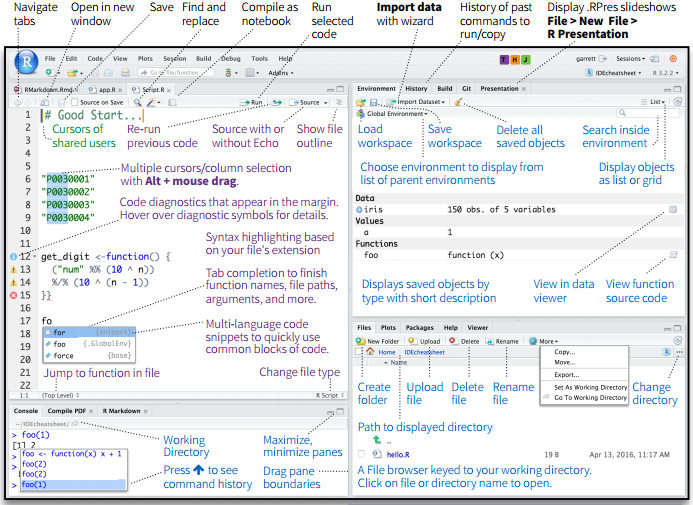
\includegraphics{figuras/rstudio_ide.png}
\caption{Fonte:
\href{https://github.com/rstudio/cheatsheets/raw/master/rstudio-ide.pdf}{RStudio
IDE Cheatsheet}}
\end{figure}

\textbf{Dicas:}

\begin{itemize}
\tightlist
\item
  Se não souber usar uma função, escreva: \texttt{?função}
\item
  As funções tem argumentos, use \textbf{TAB} para vê-los numa função
\end{itemize}

\section{IMPORTANTE}\label{importante}

\begin{itemize}
\tightlist
\item
  \textbf{TAB} no \textbf{RStudio}
\end{itemize}

Isso te ajudará a evitar coisas como: grafia errada da função, verificar
se a função existe, verificar argumentos, etc\ldots{} Use sempre!


\includegraphics[width=5.88in]{figuras/tab-key-}

\begin{itemize}
\tightlist
\item
  \textbf{Stack Overflow}
  (\href{https://stackoverflow.com/questions/tagged/r}{Veja as últimas
  das mais de 240000 (!!!) perguntas sobre R})
\end{itemize}

Melhor forma de resolver problemas! Acredite, é praticamente impossível
existir um problema que outra pessoa não tenha resolvido pelo Stack
Overflow.

\begin{quote}
\emph{Eu mesma só precisei fazer \textbf{uma} pergunta no Stack Overflow
(e acabei respondendo eu mesma depois de resolver) usando R há uns 5
anos!} - Camila.
\end{quote}

\textbf{Vamos começar!}

\chapter{R!}\label{r}

\begin{itemize}
\tightlist
\item
  Iremos focar no Linux, mas R e RStudio estão disponíveis para Windows
  e Mac também.
\item
  Documentação:
\item
  \href{http://cran.r-project.org/doc/manuals/r-release/R-intro.html}{Intro}.
\item
  \href{http://cran.r-project.org/doc/manuals/r-release/R-data.html}{I/O}.
\item
  Quer fazer um pacote?
  \href{http://cran.r-project.org/doc/manuals/r-release/R-exts.html}{Veja},
  \href{http://cran.r-project.org/doc/manuals/r-release/R-ints.html}{aqui}
  e
  \href{http://cran.r-project.org/doc/manuals/r-release/R-lang.html}{aqui}.
\item
  \href{https://stackoverflow.com/questions/tagged/r}{Stackoverflow} te
  ajudará em horas de desespero.
\end{itemize}

\section{Objetos do R}\label{objetos-do-r}

\begin{itemize}
\tightlist
\item
  Character a
\item
  Numeric 1
\item
  Integer 1
\item
  Complex 0+1i
\item
  Logical TRUE
\end{itemize}

\section{Classe}\label{classe}

\texttt{class} essa função permite ver a classe dos objetos

\section{Vetores}\label{vetores}

\begin{itemize}
\tightlist
\item
  c(``A'', ``C'', ``D'')
\item
  1:5 = c(1, 2, 3, 4, 5)
\item
  c(TRUE, FALSE)
\item
  c(1i, -1i)
\item
  c(1, ``C'', ``D'') qual é a classe???
\item
  c(1, NA, ``D'') qual é a classe???
\item
  c(1, NA, NaN) qual é a classe???
\end{itemize}

\section{Converter objetos}\label{converter-objetos}

\subsection{\texorpdfstring{\texttt{as}}{as}}\label{as}

\begin{Shaded}
\begin{Highlighting}[]
\KeywordTok{as.numeric}\NormalTok{(}\KeywordTok{c}\NormalTok{(}\DecValTok{1}\NormalTok{, }\StringTok{"C"}\NormalTok{, }\StringTok{"D"}\NormalTok{))}
\end{Highlighting}
\end{Shaded}

\begin{verbatim}
## Warning: NAs introduzidos por coerção
\end{verbatim}

\begin{verbatim}
## [1]  1 NA NA
\end{verbatim}

\hypertarget{convert_df}{\subsection{\texorpdfstring{\texttt{merge} e
\texttt{melt}}{merge e melt}}\label{convert_df}}

\section{\texorpdfstring{Matrizes e a função
\texttt{matrix}}{Matrizes e a função matrix}}\label{matrizes-e-a-funcao-matrix}

\textbf{{[}linhas, colunas{]}}

\begin{itemize}
\tightlist
\item
  Só são permitidos elementos \textbf{da mesma clase}!
\end{itemize}

Argumentos da função \texttt{matrix}

\begin{Shaded}
\begin{Highlighting}[]
\KeywordTok{args}\NormalTok{(matrix)}
\end{Highlighting}
\end{Shaded}

\begin{verbatim}
## function (data = NA, nrow = 1, ncol = 1, byrow = FALSE, dimnames = NULL) 
## NULL
\end{verbatim}

usando TAB

\begin{Shaded}
\begin{Highlighting}[]
\NormalTok{(m <-}\StringTok{ }\KeywordTok{matrix}\NormalTok{(}\DataTypeTok{data =} \DecValTok{0}\NormalTok{, }\DataTypeTok{nrow =} \DecValTok{4}\NormalTok{, }\DataTypeTok{ncol =} \DecValTok{4}\NormalTok{))}
\end{Highlighting}
\end{Shaded}

\begin{verbatim}
##      [,1] [,2] [,3] [,4]
## [1,]    0    0    0    0
## [2,]    0    0    0    0
## [3,]    0    0    0    0
## [4,]    0    0    0    0
\end{verbatim}

\begin{Shaded}
\begin{Highlighting}[]
\NormalTok{(m1 <-}\StringTok{ }\KeywordTok{matrix}\NormalTok{(}\DataTypeTok{data =} \DecValTok{1}\OperatorTok{:}\NormalTok{(}\DecValTok{4}\OperatorTok{*}\DecValTok{4}\NormalTok{), }\DataTypeTok{nrow =} \DecValTok{4}\NormalTok{, }\DataTypeTok{ncol =} \DecValTok{4}\NormalTok{))}
\end{Highlighting}
\end{Shaded}

\begin{verbatim}
##      [,1] [,2] [,3] [,4]
## [1,]    1    5    9   13
## [2,]    2    6   10   14
## [3,]    3    7   11   15
## [4,]    4    8   12   16
\end{verbatim}

\begin{Shaded}
\begin{Highlighting}[]
\KeywordTok{dim}\NormalTok{(m1)}
\end{Highlighting}
\end{Shaded}

\begin{verbatim}
## [1] 4 4
\end{verbatim}

\begin{Shaded}
\begin{Highlighting}[]
\NormalTok{(m2 <-}\StringTok{ }\KeywordTok{matrix}\NormalTok{(}\DataTypeTok{data =} \DecValTok{1}\OperatorTok{:}\NormalTok{(}\DecValTok{4}\OperatorTok{*}\DecValTok{4}\NormalTok{), }\DataTypeTok{nrow =} \DecValTok{4}\NormalTok{, }\DataTypeTok{ncol =} \DecValTok{4}\NormalTok{, }\DataTypeTok{byrow =} \OtherTok{TRUE}\NormalTok{))}
\end{Highlighting}
\end{Shaded}

\begin{verbatim}
##      [,1] [,2] [,3] [,4]
## [1,]    1    2    3    4
## [2,]    5    6    7    8
## [3,]    9   10   11   12
## [4,]   13   14   15   16
\end{verbatim}

\section{Array}\label{array}

Permite armazenar diversos elementos, com diversas dimensões. Dessa
forma, um array com duas dimensões é o mesmo que uma matriz, dessa
forma, podemos armazenar diversas matrizes dentro de um array, mas suas
dimensões são pré-estabelecidas.

\begin{Shaded}
\begin{Highlighting}[]
\KeywordTok{args}\NormalTok{(array)}
\end{Highlighting}
\end{Shaded}

\begin{verbatim}
## function (data = NA, dim = length(data), dimnames = NULL) 
## NULL
\end{verbatim}

Não esqueça do TAB

\begin{Shaded}
\begin{Highlighting}[]
\NormalTok{(a <-}\StringTok{ }\KeywordTok{array}\NormalTok{(}\DataTypeTok{data =} \DecValTok{0}\NormalTok{, }\DataTypeTok{dim =} \KeywordTok{c}\NormalTok{(}\DecValTok{1}\NormalTok{,}\DecValTok{1}\NormalTok{)))}
\end{Highlighting}
\end{Shaded}

\begin{verbatim}
##      [,1]
## [1,]    0
\end{verbatim}

\begin{Shaded}
\begin{Highlighting}[]
\KeywordTok{class}\NormalTok{(a)}
\end{Highlighting}
\end{Shaded}

\begin{verbatim}
## [1] "matrix"
\end{verbatim}

\begin{Shaded}
\begin{Highlighting}[]
\NormalTok{(a <-}\StringTok{ }\KeywordTok{array}\NormalTok{(}\DataTypeTok{data =} \DecValTok{0}\NormalTok{, }\DataTypeTok{dim =} \KeywordTok{c}\NormalTok{(}\DecValTok{1}\NormalTok{,}\DecValTok{1}\NormalTok{,}\DecValTok{1}\NormalTok{)))}
\end{Highlighting}
\end{Shaded}

\begin{verbatim}
## , , 1
## 
##      [,1]
## [1,]    0
\end{verbatim}

\begin{Shaded}
\begin{Highlighting}[]
\KeywordTok{class}\NormalTok{(a)}
\end{Highlighting}
\end{Shaded}

\begin{verbatim}
## [1] "array"
\end{verbatim}

\begin{Shaded}
\begin{Highlighting}[]
\NormalTok{(a <-}\StringTok{ }\KeywordTok{array}\NormalTok{(}\DataTypeTok{data =} \DecValTok{0}\NormalTok{, }\DataTypeTok{dim =} \KeywordTok{c}\NormalTok{(}\DecValTok{2}\NormalTok{,}\DecValTok{2}\NormalTok{,}\DecValTok{2}\NormalTok{)))}
\end{Highlighting}
\end{Shaded}

\begin{verbatim}
## , , 1
## 
##      [,1] [,2]
## [1,]    0    0
## [2,]    0    0
## 
## , , 2
## 
##      [,1] [,2]
## [1,]    0    0
## [2,]    0    0
\end{verbatim}

\begin{Shaded}
\begin{Highlighting}[]
\NormalTok{(a <-}\StringTok{ }\KeywordTok{array}\NormalTok{(}\DataTypeTok{data =} \DecValTok{0}\NormalTok{, }\DataTypeTok{dim =} \KeywordTok{c}\NormalTok{(}\DecValTok{2}\NormalTok{,}\DecValTok{4}\NormalTok{,}\DecValTok{4}\NormalTok{)))}
\end{Highlighting}
\end{Shaded}

\begin{verbatim}
## , , 1
## 
##      [,1] [,2] [,3] [,4]
## [1,]    0    0    0    0
## [2,]    0    0    0    0
## 
## , , 2
## 
##      [,1] [,2] [,3] [,4]
## [1,]    0    0    0    0
## [2,]    0    0    0    0
## 
## , , 3
## 
##      [,1] [,2] [,3] [,4]
## [1,]    0    0    0    0
## [2,]    0    0    0    0
## 
## , , 4
## 
##      [,1] [,2] [,3] [,4]
## [1,]    0    0    0    0
## [2,]    0    0    0    0
\end{verbatim}

\begin{Shaded}
\begin{Highlighting}[]
\KeywordTok{dim}\NormalTok{(a)}
\end{Highlighting}
\end{Shaded}

\begin{verbatim}
## [1] 2 4 4
\end{verbatim}

\begin{Shaded}
\begin{Highlighting}[]
\NormalTok{(a <-}\StringTok{ }\KeywordTok{array}\NormalTok{(}\DataTypeTok{data =} \DecValTok{0}\NormalTok{, }\DataTypeTok{dim =} \KeywordTok{c}\NormalTok{(}\DecValTok{2}\NormalTok{, }\DecValTok{2}\NormalTok{,}\DecValTok{2}\NormalTok{,}\DecValTok{2}\NormalTok{)))}
\end{Highlighting}
\end{Shaded}

\section{\texorpdfstring{\texttt{list}}{list}}\label{list}

Já as listas permitem que você armazene qualquer tipo de ojeto,
independente da classe, dessa forma, podemos colocar numa lista: número,
caracteres, argumentos lógicos, ou que você quiser:

\begin{Shaded}
\begin{Highlighting}[]
\KeywordTok{list}\NormalTok{(}\KeywordTok{list}\NormalTok{(}\KeywordTok{list}\NormalTok{(}\KeywordTok{list}\NormalTok{(}\DecValTok{1}\NormalTok{))))}
\end{Highlighting}
\end{Shaded}

\begin{verbatim}
## [[1]]
## [[1]][[1]]
## [[1]][[1]][[1]]
## [[1]][[1]][[1]][[1]]
## [1] 1
\end{verbatim}

Isso faz com que elas sejam bastante versáteis e sirvam para armazenar o
que você precisar, mas elas só podem ter uma dimensão, como uma fila.

\begin{Shaded}
\begin{Highlighting}[]
\NormalTok{(x <-}\StringTok{ }\KeywordTok{list}\NormalTok{(}\DecValTok{1}\NormalTok{, }\StringTok{"a"}\NormalTok{, }\OtherTok{TRUE}\NormalTok{, }\DecValTok{1} \OperatorTok{+}\StringTok{ }\NormalTok{4i))}
\end{Highlighting}
\end{Shaded}

\begin{verbatim}
## [[1]]
## [1] 1
## 
## [[2]]
## [1] "a"
## 
## [[3]]
## [1] TRUE
## 
## [[4]]
## [1] 1+4i
\end{verbatim}

\section{Tempo e Data}\label{tempo-e-data}

R também tem classes de tempo e data:

\begin{Shaded}
\begin{Highlighting}[]
\NormalTok{(a <-}\StringTok{ }\KeywordTok{ISOdate}\NormalTok{(}\DataTypeTok{year =} \DecValTok{2018}\NormalTok{, }\DataTypeTok{month =} \DecValTok{4}\NormalTok{, }\DataTypeTok{day =} \DecValTok{5}\NormalTok{))}
\end{Highlighting}
\end{Shaded}

\begin{verbatim}
## [1] "2018-04-05 12:00:00 GMT"
\end{verbatim}

\begin{Shaded}
\begin{Highlighting}[]
\KeywordTok{class}\NormalTok{(a)}
\end{Highlighting}
\end{Shaded}

\begin{verbatim}
## [1] "POSIXct" "POSIXt"
\end{verbatim}

\begin{Shaded}
\begin{Highlighting}[]
\NormalTok{(b <-}\StringTok{ }\KeywordTok{ISOdate}\NormalTok{(}\DataTypeTok{year =} \DecValTok{2018}\NormalTok{, }\DataTypeTok{month =} \DecValTok{4}\NormalTok{, }\DataTypeTok{day =} \DecValTok{5}\NormalTok{, }\DataTypeTok{tz =} \StringTok{"Americas/Sao_Paulo"}\NormalTok{))}
\end{Highlighting}
\end{Shaded}

\begin{verbatim}
## [1] "2018-04-05 12:00:00 Americas"
\end{verbatim}

Tempo

\begin{Shaded}
\begin{Highlighting}[]
\NormalTok{(d <-}\StringTok{ }\KeywordTok{ISOdatetime}\NormalTok{(}\DataTypeTok{year =} \DecValTok{2018}\NormalTok{, }\DataTypeTok{month =} \DecValTok{4}\NormalTok{, }\DataTypeTok{day =} \DecValTok{5}\NormalTok{, }\DataTypeTok{hour =} \DecValTok{0}\NormalTok{, }\DataTypeTok{min =} \DecValTok{0}\NormalTok{, }\DataTypeTok{sec =} \DecValTok{0}\NormalTok{,}
                  \DataTypeTok{tz =} \StringTok{"Americas/Sao_Paulo"}\NormalTok{))}
\end{Highlighting}
\end{Shaded}

\begin{verbatim}
## [1] "2018-04-05 Americas"
\end{verbatim}

Caso você precise, o pacote
\href{https://github.com/eddelbuettel/nanotime}{nanotime} permite
trabalhar com nano segundos.

É possível fazer sequências:

\begin{Shaded}
\begin{Highlighting}[]
\NormalTok{hoje <-}\StringTok{ }\KeywordTok{Sys.time}\NormalTok{()}
\NormalTok{(a <-}\StringTok{ }\KeywordTok{seq.POSIXt}\NormalTok{(}\DataTypeTok{from =}\NormalTok{ hoje, }\DataTypeTok{by =} \DecValTok{3600}\NormalTok{, }\DataTypeTok{length.out =} \DecValTok{24}\NormalTok{))}
\end{Highlighting}
\end{Shaded}

\begin{verbatim}
##  [1] "2018-06-01 00:38:47 -03" "2018-06-01 01:38:47 -03"
##  [3] "2018-06-01 02:38:47 -03" "2018-06-01 03:38:47 -03"
##  [5] "2018-06-01 04:38:47 -03" "2018-06-01 05:38:47 -03"
##  [7] "2018-06-01 06:38:47 -03" "2018-06-01 07:38:47 -03"
##  [9] "2018-06-01 08:38:47 -03" "2018-06-01 09:38:47 -03"
## [11] "2018-06-01 10:38:47 -03" "2018-06-01 11:38:47 -03"
## [13] "2018-06-01 12:38:47 -03" "2018-06-01 13:38:47 -03"
## [15] "2018-06-01 14:38:47 -03" "2018-06-01 15:38:47 -03"
## [17] "2018-06-01 16:38:47 -03" "2018-06-01 17:38:47 -03"
## [19] "2018-06-01 18:38:47 -03" "2018-06-01 19:38:47 -03"
## [21] "2018-06-01 20:38:47 -03" "2018-06-01 21:38:47 -03"
## [23] "2018-06-01 22:38:47 -03" "2018-06-01 23:38:47 -03"
\end{verbatim}

funções úteis: \textbf{weekdays}, \textbf{month}, \textbf{julian}

\begin{Shaded}
\begin{Highlighting}[]
\KeywordTok{weekdays}\NormalTok{(a)}
\end{Highlighting}
\end{Shaded}

\begin{verbatim}
##  [1] "sexta" "sexta" "sexta" "sexta" "sexta" "sexta" "sexta" "sexta"
##  [9] "sexta" "sexta" "sexta" "sexta" "sexta" "sexta" "sexta" "sexta"
## [17] "sexta" "sexta" "sexta" "sexta" "sexta" "sexta" "sexta" "sexta"
\end{verbatim}

\begin{Shaded}
\begin{Highlighting}[]
\KeywordTok{months}\NormalTok{(a)}
\end{Highlighting}
\end{Shaded}

\begin{verbatim}
##  [1] "junho" "junho" "junho" "junho" "junho" "junho" "junho" "junho"
##  [9] "junho" "junho" "junho" "junho" "junho" "junho" "junho" "junho"
## [17] "junho" "junho" "junho" "junho" "junho" "junho" "junho" "junho"
\end{verbatim}

\begin{Shaded}
\begin{Highlighting}[]
\KeywordTok{julian}\NormalTok{(a) }\CommentTok{#dia Juliano*}
\end{Highlighting}
\end{Shaded}

\begin{verbatim}
## Time differences in days
##  [1] 17683.15 17683.19 17683.24 17683.28 17683.32 17683.36 17683.40
##  [8] 17683.44 17683.49 17683.53 17683.57 17683.61 17683.65 17683.69
## [15] 17683.74 17683.78 17683.82 17683.86 17683.90 17683.94 17683.99
## [22] 17684.03 17684.07 17684.11
## attr(,"origin")
## [1] "1970-01-01 GMT"
\end{verbatim}

*Para mais informações: \url{https://en.wikipedia.org/wiki/Julian_day}:

\section{Fatores}\label{fatores}

Os \texttt{factors} podem ser um pouco infernais. Dê uma olhada em
\href{http://www.burns-stat.com/documents/books/the-r-inferno/}{R
INFERNO}

São variáveis que representam categorias, como por exemplo, dias da
semana.

\begin{Shaded}
\begin{Highlighting}[]
\NormalTok{a <-}\StringTok{ }\KeywordTok{seq.POSIXt}\NormalTok{(}\DataTypeTok{from =}\NormalTok{ hoje, }\DataTypeTok{by =} \DecValTok{3600}\NormalTok{, }\DataTypeTok{length.out =} \DecValTok{24}\OperatorTok{*}\DecValTok{7}\NormalTok{)}
\NormalTok{aa <-}\StringTok{ }\KeywordTok{weekdays}\NormalTok{(a)}
\KeywordTok{class}\NormalTok{(aa)}
\end{Highlighting}
\end{Shaded}

\begin{verbatim}
## [1] "character"
\end{verbatim}

\begin{Shaded}
\begin{Highlighting}[]
\KeywordTok{factor}\NormalTok{(aa)}
\end{Highlighting}
\end{Shaded}

\begin{verbatim}
##   [1] sexta   sexta   sexta   sexta   sexta   sexta   sexta   sexta  
##   [9] sexta   sexta   sexta   sexta   sexta   sexta   sexta   sexta  
##  [17] sexta   sexta   sexta   sexta   sexta   sexta   sexta   sexta  
##  [25] sábado  sábado  sábado  sábado  sábado  sábado  sábado  sábado 
##  [33] sábado  sábado  sábado  sábado  sábado  sábado  sábado  sábado 
##  [41] sábado  sábado  sábado  sábado  sábado  sábado  sábado  sábado 
##  [49] domingo domingo domingo domingo domingo domingo domingo domingo
##  [57] domingo domingo domingo domingo domingo domingo domingo domingo
##  [65] domingo domingo domingo domingo domingo domingo domingo domingo
##  [73] segunda segunda segunda segunda segunda segunda segunda segunda
##  [81] segunda segunda segunda segunda segunda segunda segunda segunda
##  [89] segunda segunda segunda segunda segunda segunda segunda segunda
##  [97] terça   terça   terça   terça   terça   terça   terça   terça  
## [105] terça   terça   terça   terça   terça   terça   terça   terça  
## [113] terça   terça   terça   terça   terça   terça   terça   terça  
## [121] quarta  quarta  quarta  quarta  quarta  quarta  quarta  quarta 
## [129] quarta  quarta  quarta  quarta  quarta  quarta  quarta  quarta 
## [137] quarta  quarta  quarta  quarta  quarta  quarta  quarta  quarta 
## [145] quinta  quinta  quinta  quinta  quinta  quinta  quinta  quinta 
## [153] quinta  quinta  quinta  quinta  quinta  quinta  quinta  quinta 
## [161] quinta  quinta  quinta  quinta  quinta  quinta  quinta  quinta 
## Levels: domingo quarta quinta sábado segunda sexta terça
\end{verbatim}

São muito úteis para regressões, plotes e resumos estatísitcos.

Olhe os \textbf{Levels}

Então:

\begin{Shaded}
\begin{Highlighting}[]
\NormalTok{ab <-}\StringTok{ }\KeywordTok{factor}\NormalTok{(}\DataTypeTok{x =}\NormalTok{ aa,}
             \DataTypeTok{levels =} \KeywordTok{c}\NormalTok{(}\StringTok{"Monday"}\NormalTok{, }\StringTok{"Tuesday"}\NormalTok{,  }\StringTok{"Wednesday"}\NormalTok{,  }\StringTok{"Thursday"}\NormalTok{,}
                        \StringTok{"Friday"}\NormalTok{, }\StringTok{"Saturday"}\NormalTok{, }\StringTok{"Sunday"}\NormalTok{))}
\KeywordTok{levels}\NormalTok{(ab)}
\end{Highlighting}
\end{Shaded}

\begin{verbatim}
## [1] "Monday"    "Tuesday"   "Wednesday" "Thursday"  "Friday"    "Saturday" 
## [7] "Sunday"
\end{verbatim}

\section{Paste!!}\label{paste}

Como concatenar, juntar, grudar arquivos, palavras, etc etc\ldots{} é
com \texttt{paste} e \texttt{paste0}. Estas funções são muito simples
mas muito úteis!!!

\begin{Shaded}
\begin{Highlighting}[]
\KeywordTok{args}\NormalTok{(paste0)}
\end{Highlighting}
\end{Shaded}

\begin{verbatim}
## function (..., collapse = NULL) 
## NULL
\end{verbatim}

\begin{Shaded}
\begin{Highlighting}[]
\KeywordTok{args}\NormalTok{(paste)}
\end{Highlighting}
\end{Shaded}

\begin{verbatim}
## function (..., sep = " ", collapse = NULL) 
## NULL
\end{verbatim}

A diferença entre \texttt{paste0} e \texttt{paste}, é que
\texttt{paste0} não tem uma separação de characteres por default, mas
\texttt{paste} usa espaço.

\begin{Shaded}
\begin{Highlighting}[]
\NormalTok{path <-}\StringTok{ }\KeywordTok{getwd}\NormalTok{()}
\NormalTok{nome <-}\StringTok{ "SeuNome"}
\KeywordTok{paste}\NormalTok{(path, nome)}
\end{Highlighting}
\end{Shaded}

\begin{verbatim}
## [1] "/home/sergio/Documentos/cursoR SeuNome"
\end{verbatim}

\begin{Shaded}
\begin{Highlighting}[]
\KeywordTok{paste0}\NormalTok{(path, nome)}
\end{Highlighting}
\end{Shaded}

\begin{verbatim}
## [1] "/home/sergio/Documentos/cursoRSeuNome"
\end{verbatim}

\begin{Shaded}
\begin{Highlighting}[]
\KeywordTok{paste}\NormalTok{(path, }\StringTok{"/"}\NormalTok{, nome)}
\end{Highlighting}
\end{Shaded}

\begin{verbatim}
## [1] "/home/sergio/Documentos/cursoR / SeuNome"
\end{verbatim}

\begin{Shaded}
\begin{Highlighting}[]
\KeywordTok{paste}\NormalTok{(path, }\StringTok{"/-/_****;;;////"}\NormalTok{, nome)}
\end{Highlighting}
\end{Shaded}

\begin{verbatim}
## [1] "/home/sergio/Documentos/cursoR /-/_****;;;//// SeuNome"
\end{verbatim}

\begin{Shaded}
\begin{Highlighting}[]
\KeywordTok{class}\NormalTok{(}\KeywordTok{paste}\NormalTok{(path, }\StringTok{"/-/_****;;;////"}\NormalTok{, nome))}
\end{Highlighting}
\end{Shaded}

\begin{verbatim}
## [1] "character"
\end{verbatim}

\begin{Shaded}
\begin{Highlighting}[]
\KeywordTok{paste0}\NormalTok{(nome, }\StringTok{"_"}\NormalTok{, }\DecValTok{1}\OperatorTok{:}\DecValTok{10}\NormalTok{) }\CommentTok{#Função vetorizada}
\end{Highlighting}
\end{Shaded}

\begin{verbatim}
##  [1] "SeuNome_1"  "SeuNome_2"  "SeuNome_3"  "SeuNome_4"  "SeuNome_5" 
##  [6] "SeuNome_6"  "SeuNome_7"  "SeuNome_8"  "SeuNome_9"  "SeuNome_10"
\end{verbatim}

\begin{Shaded}
\begin{Highlighting}[]
\KeywordTok{paste0}\NormalTok{(}\DecValTok{1}\OperatorTok{:}\DecValTok{10}\NormalTok{) }\CommentTok{#Função vetorizada}
\end{Highlighting}
\end{Shaded}

\begin{verbatim}
##  [1] "1"  "2"  "3"  "4"  "5"  "6"  "7"  "8"  "9"  "10"
\end{verbatim}

\begin{Shaded}
\begin{Highlighting}[]
\KeywordTok{class}\NormalTok{(}\KeywordTok{paste0}\NormalTok{(}\DecValTok{1}\OperatorTok{:}\DecValTok{10}\NormalTok{))}
\end{Highlighting}
\end{Shaded}

\begin{verbatim}
## [1] "character"
\end{verbatim}

\section{Substituindo caracteres}\label{substituindo-caracteres}

Vamos supor que tu vai ler um banco de dados, e uma coluna tem o
character ``BB''. Vamos supor que nessa coluna tem um numero, mas tu
precisa \textbf{remover} o simbolo ``BB'' para logo convertir para
numero. A função que vamos usar que podemos usar é \texttt{gsub}.

\begin{Shaded}
\begin{Highlighting}[]
\NormalTok{numeros <-}\StringTok{ }\DecValTok{1}\OperatorTok{:}\DecValTok{50}
\NormalTok{b <-}\StringTok{ }\KeywordTok{round}\NormalTok{(}\KeywordTok{runif}\NormalTok{(}\DataTypeTok{n =} \DecValTok{10}\NormalTok{, }\DataTypeTok{min =} \DecValTok{1}\NormalTok{, }\DataTypeTok{max =} \DecValTok{50}\NormalTok{))}
\NormalTok{numeros[b] <-}\StringTok{ }\KeywordTok{paste0}\NormalTok{(numeros, }\StringTok{"BB"}\NormalTok{)}
\end{Highlighting}
\end{Shaded}

\begin{verbatim}
## Warning in numeros[b] <- paste0(numeros, "BB"): número de itens para para
## substituir não é um múltiplo do comprimento do substituto
\end{verbatim}

\begin{Shaded}
\begin{Highlighting}[]
\NormalTok{numeros}
\end{Highlighting}
\end{Shaded}

\begin{verbatim}
##  [1] "1"    "2"    "8BB"  "7BB"  "5"    "6"    "9BB"  "8"    "9"    "10"  
## [11] "11"   "6BB"  "13"   "14"   "15"   "5BB"  "4BB"  "18"   "19"   "20"  
## [21] "21"   "22"   "23"   "24"   "25"   "26"   "2BB"  "28"   "29"   "30"  
## [31] "31"   "1BB"  "33"   "34"   "35"   "36"   "37"   "38"   "39"   "40"  
## [41] "41"   "42"   "3BB"  "44"   "10BB" "46"   "47"   "48"   "49"   "50"
\end{verbatim}

\begin{Shaded}
\begin{Highlighting}[]
\KeywordTok{args}\NormalTok{(gsub)}
\end{Highlighting}
\end{Shaded}

\begin{verbatim}
## function (pattern, replacement, x, ignore.case = FALSE, perl = FALSE, 
##     fixed = FALSE, useBytes = FALSE) 
## NULL
\end{verbatim}

\begin{Shaded}
\begin{Highlighting}[]
\NormalTok{nn <-}\StringTok{ }\KeywordTok{gsub}\NormalTok{(}\DataTypeTok{pattern =} \StringTok{"BB"}\NormalTok{, }\DataTypeTok{replacement =} \StringTok{""}\NormalTok{, }\DataTypeTok{x =}\NormalTok{ numeros)}
\KeywordTok{class}\NormalTok{(nn)}
\end{Highlighting}
\end{Shaded}

\begin{verbatim}
## [1] "character"
\end{verbatim}

\begin{Shaded}
\begin{Highlighting}[]
\KeywordTok{as.numeric}\NormalTok{(nn)}
\end{Highlighting}
\end{Shaded}

\begin{verbatim}
##  [1]  1  2  8  7  5  6  9  8  9 10 11  6 13 14 15  5  4 18 19 20 21 22 23
## [24] 24 25 26  2 28 29 30 31  1 33 34 35 36 37 38 39 40 41 42  3 44 10 46
## [47] 47 48 49 50
\end{verbatim}

\section{Substraindo caracteres}\label{substraindo-caracteres}

Agora vamos supor que temos grudado ultimo character com BB, A função
que vamos usar é \texttt{substr}:

\begin{Shaded}
\begin{Highlighting}[]
\KeywordTok{args}\NormalTok{(substr)}
\end{Highlighting}
\end{Shaded}

\begin{verbatim}
## function (x, start, stop) 
## NULL
\end{verbatim}

Com \texttt{x} é o vetor, \texttt{start} primeiro elemento em ser
reemplazado e \texttt{stop} ultimo elemento em ser reemplazado

Vamos super uma sequenciea de 1 ate 10 e tem grudados as letras BB

\begin{Shaded}
\begin{Highlighting}[]
\NormalTok{(numeros<-}\StringTok{ }\KeywordTok{paste0}\NormalTok{(}\DecValTok{1}\OperatorTok{:}\DecValTok{9}\NormalTok{, }\StringTok{"BB"}\NormalTok{))}
\end{Highlighting}
\end{Shaded}

\begin{verbatim}
## [1] "1BB" "2BB" "3BB" "4BB" "5BB" "6BB" "7BB" "8BB" "9BB"
\end{verbatim}

Para remover os ultimos dois characters sería:

\begin{Shaded}
\begin{Highlighting}[]
\KeywordTok{substr}\NormalTok{(numeros, }\DecValTok{0}\NormalTok{, }\DecValTok{1}\NormalTok{)}
\end{Highlighting}
\end{Shaded}

\begin{verbatim}
## [1] "1" "2" "3" "4" "5" "6" "7" "8" "9"
\end{verbatim}

\begin{Shaded}
\begin{Highlighting}[]
\KeywordTok{substr}\NormalTok{(numeros, }\DecValTok{2}\NormalTok{, }\DecValTok{3}\NormalTok{)}
\end{Highlighting}
\end{Shaded}

\begin{verbatim}
## [1] "BB" "BB" "BB" "BB" "BB" "BB" "BB" "BB" "BB"
\end{verbatim}

\section{Data.frames}\label{data.frames}

\emph{lembre ?data.frame}

Lembram uma planilha EXCEL\ldots{} Mais ou menos

É uma classe bem especial, tem elementos de matriz mas o modo é lista

\begin{Shaded}
\begin{Highlighting}[]
\KeywordTok{args}\NormalTok{(data.frame)}
\end{Highlighting}
\end{Shaded}

\begin{verbatim}
## function (..., row.names = NULL, check.rows = FALSE, check.names = TRUE, 
##     fix.empty.names = TRUE, stringsAsFactors = default.stringsAsFactors()) 
## NULL
\end{verbatim}

\begin{Shaded}
\begin{Highlighting}[]
\NormalTok{(df <-}\StringTok{ }\KeywordTok{data.frame}\NormalTok{(}\DataTypeTok{a =} \DecValTok{1}\OperatorTok{:}\DecValTok{3}\NormalTok{))}
\end{Highlighting}
\end{Shaded}

\begin{verbatim}
##   a
## 1 1
## 2 2
## 3 3
\end{verbatim}

\begin{Shaded}
\begin{Highlighting}[]
\KeywordTok{names}\NormalTok{(df)}
\end{Highlighting}
\end{Shaded}

\begin{verbatim}
## [1] "a"
\end{verbatim}

\begin{Shaded}
\begin{Highlighting}[]
\KeywordTok{class}\NormalTok{(df)}
\end{Highlighting}
\end{Shaded}

\begin{verbatim}
## [1] "data.frame"
\end{verbatim}

\begin{Shaded}
\begin{Highlighting}[]
\KeywordTok{mode}\NormalTok{(df)}
\end{Highlighting}
\end{Shaded}

\begin{verbatim}
## [1] "list"
\end{verbatim}

Podemos utilizar para armazenar dados, sendo que um data.frame é sempre
composto por vetores com comprimento IGUAL

\begin{Shaded}
\begin{Highlighting}[]
\KeywordTok{nrow}\NormalTok{(df)}
\end{Highlighting}
\end{Shaded}

\begin{verbatim}
## [1] 3
\end{verbatim}

\begin{Shaded}
\begin{Highlighting}[]
\KeywordTok{ncol}\NormalTok{(df)}
\end{Highlighting}
\end{Shaded}

\begin{verbatim}
## [1] 1
\end{verbatim}

\begin{Shaded}
\begin{Highlighting}[]
\KeywordTok{dim}\NormalTok{(df)}
\end{Highlighting}
\end{Shaded}

\begin{verbatim}
## [1] 3 1
\end{verbatim}

Algumas operações que pode fazer com data.frames são:

\begin{itemize}
\tightlist
\item
  rbind: une verticalmente (por linhas\ldots{} row) duas data.frames
\item
  cbind: Une horizontalmente duas data.frames por colunas
\item
  merge: Une horizontalmente data.frames por coincidencia de dados nas
  colunas
\end{itemize}

faza?

\begin{Shaded}
\begin{Highlighting}[]
\NormalTok{?rbind}
\end{Highlighting}
\end{Shaded}

\begin{verbatim}
## Help on topic 'rbind' was found in the following packages:
## 
##   Package               Library
##   base                  /usr/lib/R/library
##   data.table            /home/sergio/R/x86_64-pc-linux-gnu-library/3.4
## 
## 
## Using the first match ...
\end{verbatim}

\begin{Shaded}
\begin{Highlighting}[]
\NormalTok{?cbind}
\NormalTok{?merge}
\end{Highlighting}
\end{Shaded}

\begin{verbatim}
## Help on topic 'merge' was found in the following packages:
## 
##   Package               Library
##   sp                    /home/sergio/R/x86_64-pc-linux-gnu-library/3.4
##   base                  /usr/lib/R/library
##   raster                /home/sergio/R/x86_64-pc-linux-gnu-library/3.4
##   data.table            /home/sergio/R/x86_64-pc-linux-gnu-library/3.4
## 
## 
## Using the first match ...
\end{verbatim}

Exemplo:

\begin{Shaded}
\begin{Highlighting}[]
\NormalTok{a <-}\StringTok{ }\KeywordTok{data.frame}\NormalTok{(}\DataTypeTok{id =} \KeywordTok{c}\NormalTok{(}\StringTok{"a"}\NormalTok{, }\StringTok{"b"}\NormalTok{, }\StringTok{"c"}\NormalTok{))}
\NormalTok{b <-}\StringTok{ }\KeywordTok{data.frame}\NormalTok{(}\DataTypeTok{id =} \KeywordTok{c}\NormalTok{(}\StringTok{"Z"}\NormalTok{, }\StringTok{"b"}\NormalTok{, }\StringTok{"D"}\NormalTok{))}
\KeywordTok{merge}\NormalTok{(}\DataTypeTok{x =}\NormalTok{ a, }\DataTypeTok{y =}\NormalTok{ b, }\DataTypeTok{by =} \StringTok{"id"}\NormalTok{)}
\end{Highlighting}
\end{Shaded}

\begin{verbatim}
##   id
## 1  b
\end{verbatim}

\chapter{Importando e Exportando
Dados}\label{importando-e-exportando-dados}

\section{Data Frames}\label{data-frames}

Probabelmente um dos promeiros objetos que vamos usar quando começamos
usar R. Pensa num data-frame como uma planilha de Libreoffice (o excel).
Os data-frame pode ser criaos como foi visto na seção anterior. O
principal, é que temos varias funções para ler data-frames no R, entre
elas

\begin{itemize}
\tightlist
\item
  read.csv
\item
  read.csv2
\item
  read.table
\end{itemize}

Agora vamos a ler dados do repositorio usando read.table, mas primeiro
vamos lembrar que se tu precisar ver a ajuda da função, tem que escrever
no R \texttt{?read.table}. Então, agora vamos ver os argumentos da
função:

\begin{Shaded}
\begin{Highlighting}[]
\KeywordTok{args}\NormalTok{(read.table)}
\end{Highlighting}
\end{Shaded}

\begin{verbatim}
## function (file, header = FALSE, sep = "", quote = "\"'", dec = ".", 
##     numerals = c("allow.loss", "warn.loss", "no.loss"), row.names, 
##     col.names, as.is = !stringsAsFactors, na.strings = "NA", 
##     colClasses = NA, nrows = -1, skip = 0, check.names = TRUE, 
##     fill = !blank.lines.skip, strip.white = FALSE, blank.lines.skip = TRUE, 
##     comment.char = "#", allowEscapes = FALSE, flush = FALSE, 
##     stringsAsFactors = default.stringsAsFactors(), fileEncoding = "", 
##     encoding = "unknown", text, skipNul = FALSE) 
## NULL
\end{verbatim}

Aqui vem-se os valores default dos argumentos da função
\texttt{read.table}. O terceiro argumento é sep, com valores por default
= ``''.

\begin{Shaded}
\begin{Highlighting}[]
\NormalTok{df <-}\StringTok{ }\KeywordTok{read.table}\NormalTok{(}\StringTok{"https://raw.githubusercontent.com/ibarraespinosa/cursoR/master/dados/NOXIPEN2014.txt"}\NormalTok{)}
\end{Highlighting}
\end{Shaded}

Agora vamos usar a funções \texttt{head} and \texttt{tail} para ver as
primeiras e as ultimas 6 linhas do data-frame.

\begin{Shaded}
\begin{Highlighting}[]
\KeywordTok{head}\NormalTok{(df)}
\end{Highlighting}
\end{Shaded}

\begin{verbatim}
##   TipodeRede TipodeMonitoramento            Tipo       Data  Hora
## 2 Automático              CETESB Dados Primários 01/01/2014 01:00
## 3 Automático              CETESB Dados Primários 01/01/2014 02:00
## 4 Automático              CETESB Dados Primários 01/01/2014 03:00
## 5 Automático              CETESB Dados Primários 01/01/2014 04:00
## 6 Automático              CETESB Dados Primários 01/01/2014 05:00
## 7 Automático              CETESB Dados Primários 01/01/2014 06:00
##   CodigoEstação                NomeEstação              NomeParâmetro
## 2            95 Cid.Universitária-USP-Ipen NOx (Óxidos de Nitrogênio)
## 3            95 Cid.Universitária-USP-Ipen NOx (Óxidos de Nitrogênio)
## 4            95 Cid.Universitária-USP-Ipen NOx (Óxidos de Nitrogênio)
## 5            95 Cid.Universitária-USP-Ipen NOx (Óxidos de Nitrogênio)
## 6            95 Cid.Universitária-USP-Ipen NOx (Óxidos de Nitrogênio)
## 7            95 Cid.Universitária-USP-Ipen NOx (Óxidos de Nitrogênio)
##   UnidadedeMedida MediaHoraria MediaMovel Valido
## 2             ppb            9          -    Não
## 3             ppb            9          -    Sim
## 4             ppb            5          -    Sim
## 5             ppb            4          -    Sim
## 6             ppb            5          -    Sim
## 7             ppb            5          -    Sim
\end{verbatim}

\begin{Shaded}
\begin{Highlighting}[]
\KeywordTok{tail}\NormalTok{(df)}
\end{Highlighting}
\end{Shaded}

\begin{verbatim}
##      TipodeRede TipodeMonitoramento            Tipo       Data  Hora
## 8577 Automático              CETESB Dados Primários 01/01/2015 19:00
## 8578 Automático              CETESB Dados Primários 01/01/2015 20:00
## 8579 Automático              CETESB Dados Primários 01/01/2015 21:00
## 8580 Automático              CETESB Dados Primários 01/01/2015 22:00
## 8581 Automático              CETESB Dados Primários 01/01/2015 23:00
## 8582 Automático              CETESB Dados Primários 01/01/2015 24:00
##      CodigoEstação                NomeEstação              NomeParâmetro
## 8577            95 Cid.Universitária-USP-Ipen NOx (Óxidos de Nitrogênio)
## 8578            95 Cid.Universitária-USP-Ipen NOx (Óxidos de Nitrogênio)
## 8579            95 Cid.Universitária-USP-Ipen NOx (Óxidos de Nitrogênio)
## 8580            95 Cid.Universitária-USP-Ipen NOx (Óxidos de Nitrogênio)
## 8581            95 Cid.Universitária-USP-Ipen NOx (Óxidos de Nitrogênio)
## 8582            95 Cid.Universitária-USP-Ipen NOx (Óxidos de Nitrogênio)
##      UnidadedeMedida MediaHoraria MediaMovel Valido
## 8577             ppb            3          -    Sim
## 8578             ppb            8          -    Sim
## 8579             ppb           11          -    Sim
## 8580             ppb           11          -    Sim
## 8581             ppb           16          -    Sim
## 8582             ppb           NA          -    Sim
\end{verbatim}

Agora vamos ler os mesmos dados com outro formato e testar e read.table
funciona do mesmo jeito

\begin{Shaded}
\begin{Highlighting}[]
\NormalTok{df2 <-}\StringTok{ }\KeywordTok{read.table}\NormalTok{(}\StringTok{"https://raw.githubusercontent.com/ibarraespinosa/cursoR/master/dados/NOXIPEN2014v2.txt"}\NormalTok{)}
\CommentTok{# Error in scan(file = file, what = what, sep = sep, quote = quote, dec = dec, : }
\CommentTok{# linha 1 não tinha 6 elementos}
\end{Highlighting}
\end{Shaded}

Vemos a mensagem de error, mas o que quer dizer.

\textbf{Se tu recever um banco de dados tipo .txt e quer abrir no
R\ldots{} ABRE ELE COM BLOCO DE NOTAS PRIMEIRO!!!}

O primeiro arquivo:

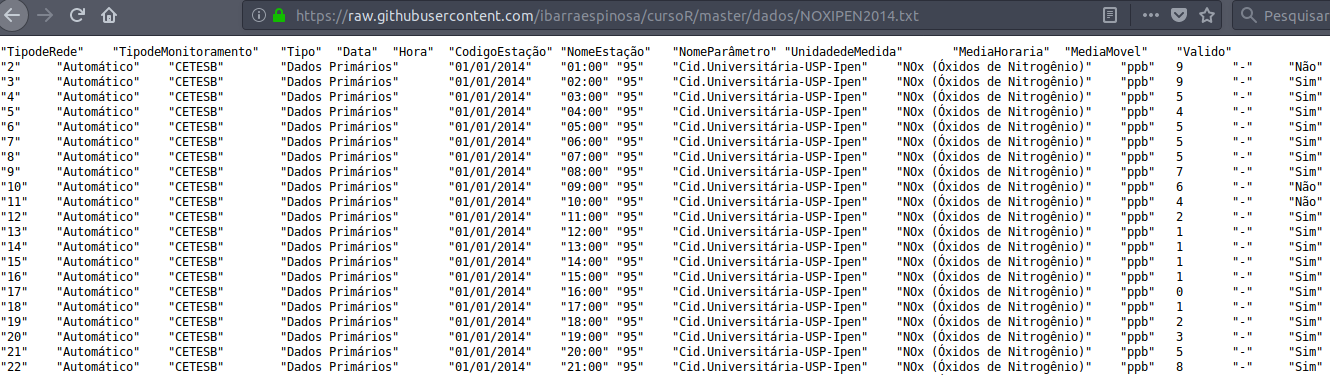
\includegraphics[width=18.47in]{figuras/f1}

O segundo arquivo é:

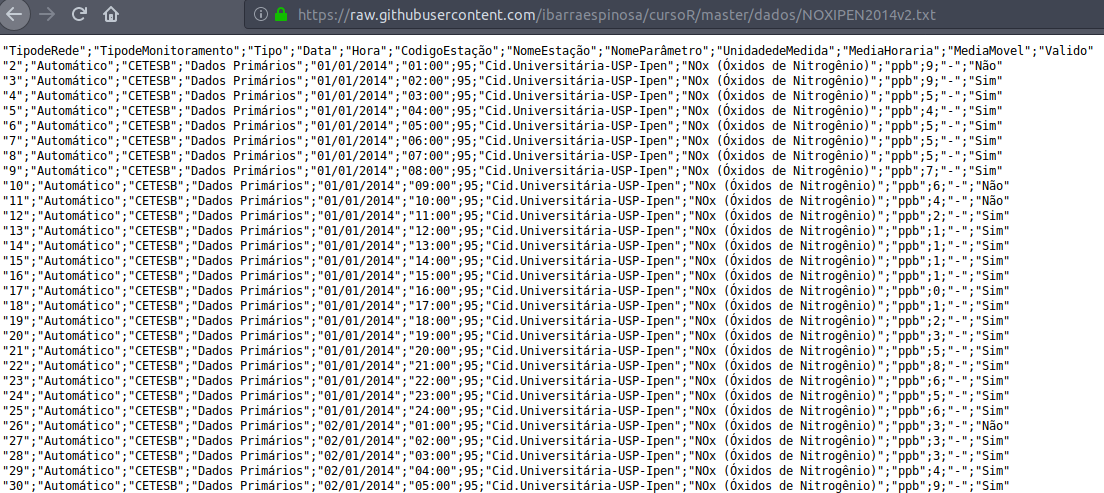
\includegraphics[width=15.33in]{figuras/f2}

qual é a diferença?

Como vemos o segundo arquivo tem separação de ``;'', entao, temos que
lero arquivo assim:

\begin{Shaded}
\begin{Highlighting}[]
\NormalTok{df2 <-}\StringTok{ }\KeywordTok{read.table}\NormalTok{(}\StringTok{"https://raw.githubusercontent.com/ibarraespinosa/cursoR/master/dados/NOXIPEN2014v2.txt"}\NormalTok{, }\DataTypeTok{sep =} \StringTok{";"}\NormalTok{)}
\KeywordTok{head}\NormalTok{(df2)}
\end{Highlighting}
\end{Shaded}

\begin{verbatim}
##   TipodeRede TipodeMonitoramento            Tipo       Data  Hora
## 2 Automático              CETESB Dados Primários 01/01/2014 01:00
## 3 Automático              CETESB Dados Primários 01/01/2014 02:00
## 4 Automático              CETESB Dados Primários 01/01/2014 03:00
## 5 Automático              CETESB Dados Primários 01/01/2014 04:00
## 6 Automático              CETESB Dados Primários 01/01/2014 05:00
## 7 Automático              CETESB Dados Primários 01/01/2014 06:00
##   CodigoEstação                NomeEstação              NomeParâmetro
## 2            95 Cid.Universitária-USP-Ipen NOx (Óxidos de Nitrogênio)
## 3            95 Cid.Universitária-USP-Ipen NOx (Óxidos de Nitrogênio)
## 4            95 Cid.Universitária-USP-Ipen NOx (Óxidos de Nitrogênio)
## 5            95 Cid.Universitária-USP-Ipen NOx (Óxidos de Nitrogênio)
## 6            95 Cid.Universitária-USP-Ipen NOx (Óxidos de Nitrogênio)
## 7            95 Cid.Universitária-USP-Ipen NOx (Óxidos de Nitrogênio)
##   UnidadedeMedida MediaHoraria MediaMovel Valido
## 2             ppb            9          -    Não
## 3             ppb            9          -    Sim
## 4             ppb            5          -    Sim
## 5             ppb            4          -    Sim
## 6             ppb            5          -    Sim
## 7             ppb            5          -    Sim
\end{verbatim}

\begin{Shaded}
\begin{Highlighting}[]
\KeywordTok{tail}\NormalTok{(df2)}
\end{Highlighting}
\end{Shaded}

\begin{verbatim}
##      TipodeRede TipodeMonitoramento            Tipo       Data  Hora
## 8577 Automático              CETESB Dados Primários 01/01/2015 19:00
## 8578 Automático              CETESB Dados Primários 01/01/2015 20:00
## 8579 Automático              CETESB Dados Primários 01/01/2015 21:00
## 8580 Automático              CETESB Dados Primários 01/01/2015 22:00
## 8581 Automático              CETESB Dados Primários 01/01/2015 23:00
## 8582 Automático              CETESB Dados Primários 01/01/2015 24:00
##      CodigoEstação                NomeEstação              NomeParâmetro
## 8577            95 Cid.Universitária-USP-Ipen NOx (Óxidos de Nitrogênio)
## 8578            95 Cid.Universitária-USP-Ipen NOx (Óxidos de Nitrogênio)
## 8579            95 Cid.Universitária-USP-Ipen NOx (Óxidos de Nitrogênio)
## 8580            95 Cid.Universitária-USP-Ipen NOx (Óxidos de Nitrogênio)
## 8581            95 Cid.Universitária-USP-Ipen NOx (Óxidos de Nitrogênio)
## 8582            95 Cid.Universitária-USP-Ipen NOx (Óxidos de Nitrogênio)
##      UnidadedeMedida MediaHoraria MediaMovel Valido
## 8577             ppb            3          -    Sim
## 8578             ppb            8          -    Sim
## 8579             ppb           11          -    Sim
## 8580             ppb           11          -    Sim
## 8581             ppb           16          -    Sim
## 8582             ppb           NA          -    Sim
\end{verbatim}

\textbf{Qua dificultades tu já enfrentou importando dados?}

\section{BASE}\label{base}

\subsection{\texorpdfstring{Exportando texto com
\texttt{write.table}}{Exportando texto com write.table}}\label{exportando-texto-com-write.table}

Exportar é bem facil, mas se sabemos os argumentos das funções, vai ser
mais eficiente ainda. Vamos \texttt{write.table}

\begin{Shaded}
\begin{Highlighting}[]
\KeywordTok{args}\NormalTok{(write.table)}
\end{Highlighting}
\end{Shaded}

\begin{verbatim}
## function (x, file = "", append = FALSE, quote = TRUE, sep = " ", 
##     eol = "\n", na = "NA", dec = ".", row.names = TRUE, col.names = TRUE, 
##     qmethod = c("escape", "double"), fileEncoding = "") 
## NULL
\end{verbatim}

Se temos um data-frame com colunas de classe character,
\texttt{quote\ =\ TRUE} quer dizer que o arquivo de texto resultante vai
ter aspas nas colunas de caracter.

\texttt{sep} é como vão ser separadas as colunas. Se tu quer abrir o
arquivo com Excel, poderia separar com ``,'', ``;'', " ``,''\t``\ldots{}
Depende como tu quer.

eol quer dizer \emph{end of line}, e é para ver a forma de colocar o
``end of line''

\textbf{row.names}.. esta TRUE mas SEMPRE SEMPRE SEMPRE COLOCA:

\textbf{row.names = FALSE}. Se não, R vai adiiconar uma coluna com os
indices das linhas\ldots{}.

col.names se tu quer o nome nas colunas\ldots{}

\textbf{PRATICA!}

\subsection{\texorpdfstring{Exportando objetos com
\texttt{save}}{Exportando objetos com save}}\label{exportando-objetos-com-save}

\begin{Shaded}
\begin{Highlighting}[]
\KeywordTok{args}\NormalTok{(save)}
\end{Highlighting}
\end{Shaded}

\begin{verbatim}
## function (..., list = character(), file = stop("'file' must be specified"), 
##     ascii = FALSE, version = NULL, envir = parent.frame(), compress = isTRUE(!ascii), 
##     compression_level, eval.promises = TRUE, precheck = TRUE) 
## NULL
\end{verbatim}

\texttt{save} salva o objeto com a extensão .rda. Para carregar de volta
o objeto, tem que ser feito com a função \texttt{load}

\begin{Shaded}
\begin{Highlighting}[]
\KeywordTok{args}\NormalTok{(load)}
\end{Highlighting}
\end{Shaded}

\begin{verbatim}
## function (file, envir = parent.frame(), verbose = FALSE) 
## NULL
\end{verbatim}

O que pode ser ruim, porque as vezes tu esqueceu o nome do objeto no
ambiente de R. Por exemplo, tu salvou o arquivo

\begin{Shaded}
\begin{Highlighting}[]
\KeywordTok{save}\NormalTok{(frenteFria, }\DataTypeTok{file =} \StringTok{"FrenteQuente.rda"}\NormalTok{)}
\end{Highlighting}
\end{Shaded}

logo tu carrega

\begin{Shaded}
\begin{Highlighting}[]
\KeywordTok{load}\NormalTok{(}\StringTok{"FrenteQuente.rda"}\NormalTok{)}
\end{Highlighting}
\end{Shaded}

acreditando que vai ter tua frente quente, mas o nome do objeto no
ambiente de R é frenteDria\ldots{} então, tem que ficar de olho, e como
somos imperfeito, vai dar merda\ldots{}.

O melhor da função é que permite salvar com tipos de compressão, por
exemplo compress = ``xz''.

\subsection{\texorpdfstring{Exportando objetos com
\texttt{saveRDS}}{Exportando objetos com saveRDS}}\label{exportando-objetos-com-saverds}

Esta é uma das minhas funçoes favoritas no R

\begin{Shaded}
\begin{Highlighting}[]
\KeywordTok{args}\NormalTok{(saveRDS)}
\end{Highlighting}
\end{Shaded}

\begin{verbatim}
## function (object, file = "", ascii = FALSE, version = NULL, compress = TRUE, 
##     refhook = NULL) 
## NULL
\end{verbatim}

e

\begin{Shaded}
\begin{Highlighting}[]
\KeywordTok{args}\NormalTok{(readRDS)}
\end{Highlighting}
\end{Shaded}

\begin{verbatim}
## function (file, refhook = NULL) 
## NULL
\end{verbatim}

Tu consegue salvar o objeto R de forma serializada e compactada com o
argumento \texttt{compress} mas o melhor é quando vai chamar o objeto de
volta ao R. Agora tu usa o \texttt{readRDS} e coloca o nome que tu
quiser.

\begin{Shaded}
\begin{Highlighting}[]
\KeywordTok{saveRDS}\NormalTok{(FrenteQuente, }\StringTok{"FrenteQuente.rds"}\NormalTok{)}
\end{Highlighting}
\end{Shaded}

\begin{Shaded}
\begin{Highlighting}[]
\NormalTok{frenteQ <-}\StringTok{ }\KeywordTok{readRDS}\NormalTok{(}\StringTok{"FremteQuente.rds"}\NormalTok{)}
\end{Highlighting}
\end{Shaded}

\hypertarget{processing_dfs}{\subsection{Processando nossa
data-frame}\label{processing_dfs}}

Tem numeroas formas e pacotes para ordenar, arrangiar (Arrange), mutar e
cambiar as data-frames. As mais conhecidas são provablemente do universe
\emph{tidyverse} com o famoso pacote \emph{dplyr}. Mas, nesta curso
vamos focar em \textbf{base}.

Vamos então revisar a classe de cada columna do nosso data-frame com a
função \texttt{sapply}, apresentada em outro capitulo, mas se quiser, da
uma olhada em \texttt{?sapply}.

\begin{Shaded}
\begin{Highlighting}[]
\KeywordTok{sapply}\NormalTok{(df, class)}
\end{Highlighting}
\end{Shaded}

\begin{verbatim}
##          TipodeRede TipodeMonitoramento                Tipo 
##            "factor"            "factor"            "factor" 
##                Data                Hora       CodigoEstação 
##            "factor"            "factor"           "integer" 
##         NomeEstação       NomeParâmetro     UnidadedeMedida 
##            "factor"            "factor"            "factor" 
##        MediaHoraria          MediaMovel              Valido 
##           "integer"            "factor"            "factor"
\end{verbatim}

Quando nos trabalhamos com series de tempo, é importante ter a variabel
de tempo reconhecida como ``tempo'', especificamente como classe
``POSIXct''. Mas, a classe de Data é ``factor'' e de Hora tambem
``factor'', o que é ruim. Então, vamos criar uma variabel de tempo mais
standard com formato 2018-06-01 00:38:51.

Para isso temos que grudar as variabel Data e Hora. Faremios isso numa
nova varaibel chamada tempo\_char, adicionando ela diretamente no
\texttt{df} com o cifrão DOLLAR \$. O grude pode ser feito com as
funções \texttt{paste} ou \texttt{paste0}.

\begin{Shaded}
\begin{Highlighting}[]
\NormalTok{df}\OperatorTok{$}\NormalTok{tempo_char <-}\StringTok{ }\KeywordTok{paste}\NormalTok{(df}\OperatorTok{$}\NormalTok{Data, df}\OperatorTok{$}\NormalTok{Hora)}
\KeywordTok{head}\NormalTok{(df}\OperatorTok{$}\NormalTok{tempo_char)}
\end{Highlighting}
\end{Shaded}

\begin{verbatim}
## [1] "01/01/2014 01:00" "01/01/2014 02:00" "01/01/2014 03:00"
## [4] "01/01/2014 04:00" "01/01/2014 05:00" "01/01/2014 06:00"
\end{verbatim}

\begin{Shaded}
\begin{Highlighting}[]
\KeywordTok{class}\NormalTok{(df}\OperatorTok{$}\NormalTok{tempo_char)}
\end{Highlighting}
\end{Shaded}

\begin{verbatim}
## [1] "character"
\end{verbatim}

Esta melhorando mas ainda tem clase character.

Para convertir a nossa classe POSIXct podemos usar a função
\texttt{as.POSIXct} (olha \texttt{as.POSIXct}). Seus argumentos são:

\begin{Shaded}
\begin{Highlighting}[]
\KeywordTok{args}\NormalTok{(as.POSIXct)}
\end{Highlighting}
\end{Shaded}

\begin{verbatim}
## function (x, tz = "", ...) 
## NULL
\end{verbatim}

Então, vamos criar outra variabel tempo o formato POSIXct

\begin{Shaded}
\begin{Highlighting}[]
\NormalTok{df}\OperatorTok{$}\NormalTok{tempo <-}\StringTok{ }\KeywordTok{as.POSIXct}\NormalTok{(}\DataTypeTok{x =}\NormalTok{ df}\OperatorTok{$}\NormalTok{tempo_char, }\DataTypeTok{tz =} \StringTok{"Americas/Sao_Paulo"}\NormalTok{, }
                       \DataTypeTok{format =} \StringTok{"%d/%m/%Y %H:%M"}\NormalTok{)}
\KeywordTok{head}\NormalTok{(df}\OperatorTok{$}\NormalTok{tempo)}
\end{Highlighting}
\end{Shaded}

\begin{verbatim}
## [1] "2014-01-01 01:00:00 Americas" "2014-01-01 02:00:00 Americas"
## [3] "2014-01-01 03:00:00 Americas" "2014-01-01 04:00:00 Americas"
## [5] "2014-01-01 05:00:00 Americas" "2014-01-01 06:00:00 Americas"
\end{verbatim}

\begin{Shaded}
\begin{Highlighting}[]
\KeywordTok{class}\NormalTok{(df}\OperatorTok{$}\NormalTok{tempo)}
\end{Highlighting}
\end{Shaded}

\begin{verbatim}
## [1] "POSIXct" "POSIXt"
\end{verbatim}

Agora, vamos a extraer os dias da semana do tempo, mes e dia juliano:

\begin{Shaded}
\begin{Highlighting}[]
\NormalTok{df}\OperatorTok{$}\NormalTok{weekdays <-}\StringTok{ }\KeywordTok{format}\NormalTok{(df}\OperatorTok{$}\NormalTok{tempo, }\StringTok{"%A"}\NormalTok{)}
\KeywordTok{head}\NormalTok{(df}\OperatorTok{$}\NormalTok{weekdays)}
\end{Highlighting}
\end{Shaded}

\begin{verbatim}
## [1] "quarta" "quarta" "quarta" "quarta" "quarta" "quarta"
\end{verbatim}

\begin{Shaded}
\begin{Highlighting}[]
\NormalTok{df}\OperatorTok{$}\NormalTok{mes <-}\StringTok{ }\KeywordTok{format}\NormalTok{(df}\OperatorTok{$}\NormalTok{tempo, }\StringTok{"%B"}\NormalTok{)}
\KeywordTok{head}\NormalTok{(df}\OperatorTok{$}\NormalTok{mes)}
\end{Highlighting}
\end{Shaded}

\begin{verbatim}
## [1] "janeiro" "janeiro" "janeiro" "janeiro" "janeiro" "janeiro"
\end{verbatim}

\begin{Shaded}
\begin{Highlighting}[]
\NormalTok{df}\OperatorTok{$}\NormalTok{diajuliano <-}\StringTok{ }\KeywordTok{julian}\NormalTok{(df}\OperatorTok{$}\NormalTok{tempo)}
\KeywordTok{head}\NormalTok{(df}\OperatorTok{$}\NormalTok{diajuliano)}
\end{Highlighting}
\end{Shaded}

\begin{verbatim}
## Time differences in days
## [1] 16071.04 16071.08 16071.12 16071.17 16071.21 16071.25
\end{verbatim}

\begin{Shaded}
\begin{Highlighting}[]
\NormalTok{df}\OperatorTok{$}\NormalTok{ano <-}\StringTok{ }\KeywordTok{format}\NormalTok{(df}\OperatorTok{$}\NormalTok{tempo, }\StringTok{"%Y"}\NormalTok{)}
\end{Highlighting}
\end{Shaded}

\subsection{aggregate}\label{aggregate}

Vamos a carregar a nossa data.frame. Primero uma olhada

\begin{Shaded}
\begin{Highlighting}[]
\KeywordTok{head}\NormalTok{(df)}
\end{Highlighting}
\end{Shaded}

\begin{verbatim}
##   TipodeRede TipodeMonitoramento            Tipo       Data  Hora
## 2 Automático              CETESB Dados Primários 01/01/2014 01:00
## 3 Automático              CETESB Dados Primários 01/01/2014 02:00
## 4 Automático              CETESB Dados Primários 01/01/2014 03:00
## 5 Automático              CETESB Dados Primários 01/01/2014 04:00
## 6 Automático              CETESB Dados Primários 01/01/2014 05:00
## 7 Automático              CETESB Dados Primários 01/01/2014 06:00
##   CodigoEstação                NomeEstação              NomeParâmetro
## 2            95 Cid.Universitária-USP-Ipen NOx (Óxidos de Nitrogênio)
## 3            95 Cid.Universitária-USP-Ipen NOx (Óxidos de Nitrogênio)
## 4            95 Cid.Universitária-USP-Ipen NOx (Óxidos de Nitrogênio)
## 5            95 Cid.Universitária-USP-Ipen NOx (Óxidos de Nitrogênio)
## 6            95 Cid.Universitária-USP-Ipen NOx (Óxidos de Nitrogênio)
## 7            95 Cid.Universitária-USP-Ipen NOx (Óxidos de Nitrogênio)
##   UnidadedeMedida MediaHoraria MediaMovel Valido       tempo_char
## 2             ppb            9          -    Não 01/01/2014 01:00
## 3             ppb            9          -    Sim 01/01/2014 02:00
## 4             ppb            5          -    Sim 01/01/2014 03:00
## 5             ppb            4          -    Sim 01/01/2014 04:00
## 6             ppb            5          -    Sim 01/01/2014 05:00
## 7             ppb            5          -    Sim 01/01/2014 06:00
##                 tempo weekdays     mes    diajuliano  ano
## 2 2014-01-01 01:00:00   quarta janeiro 16071.04 days 2014
## 3 2014-01-01 02:00:00   quarta janeiro 16071.08 days 2014
## 4 2014-01-01 03:00:00   quarta janeiro 16071.12 days 2014
## 5 2014-01-01 04:00:00   quarta janeiro 16071.17 days 2014
## 6 2014-01-01 05:00:00   quarta janeiro 16071.21 days 2014
## 7 2014-01-01 06:00:00   quarta janeiro 16071.25 days 2014
\end{verbatim}

Poderiamos calcular a media horaria por dia da semana. Então:

\begin{Shaded}
\begin{Highlighting}[]
\NormalTok{dff <-}\StringTok{ }\KeywordTok{aggregate}\NormalTok{(df}\OperatorTok{$}\NormalTok{MediaHoraria, }\DataTypeTok{by =} \KeywordTok{list}\NormalTok{(df}\OperatorTok{$}\NormalTok{weekdays), sum, }\DataTypeTok{na.rm =}\NormalTok{ T)}
\NormalTok{dff}
\end{Highlighting}
\end{Shaded}

\begin{verbatim}
##   Group.1     x
## 1 domingo 20327
## 2  quarta 40180
## 3  quinta 41199
## 4  sábado 32298
## 5 segunda 34057
## 6   sexta 42558
## 7   terça 37904
\end{verbatim}

\begin{Shaded}
\begin{Highlighting}[]
\KeywordTok{names}\NormalTok{(dff) <-}\StringTok{ }\KeywordTok{c}\NormalTok{(}\StringTok{"dias"}\NormalTok{, }\StringTok{"MediaHoraria"}\NormalTok{)}
\end{Highlighting}
\end{Shaded}

\begin{Shaded}
\begin{Highlighting}[]
\NormalTok{dff}\OperatorTok{$}\NormalTok{sd <-}\StringTok{ }\KeywordTok{aggregate}\NormalTok{(df}\OperatorTok{$}\NormalTok{MediaHoraria, }
                    \DataTypeTok{by =} \KeywordTok{list}\NormalTok{(df}\OperatorTok{$}\NormalTok{weekdays), }
\NormalTok{                    sum, }\DataTypeTok{na.rm =}\NormalTok{ T)}\OperatorTok{$}\NormalTok{x}
\NormalTok{dff}
\end{Highlighting}
\end{Shaded}

\begin{verbatim}
##      dias MediaHoraria    sd
## 1 domingo        20327 20327
## 2  quarta        40180 40180
## 3  quinta        41199 41199
## 4  sábado        32298 32298
## 5 segunda        34057 34057
## 6   sexta        42558 42558
## 7   terça        37904 37904
\end{verbatim}

\subsection{subset}\label{subset}

Como poderiamos escolher só o mes de janeiro??

\begin{Shaded}
\begin{Highlighting}[]
\CommentTok{#[     LINHAS    ,  COLUNAS   ]}
\KeywordTok{head}\NormalTok{(df[df}\OperatorTok{$}\NormalTok{mes }\OperatorTok{==}\StringTok{ "janeiro"}\NormalTok{, ]) }\CommentTok{#TODAS AS COLUNAS}
\end{Highlighting}
\end{Shaded}

\begin{verbatim}
##   TipodeRede TipodeMonitoramento            Tipo       Data  Hora
## 2 Automático              CETESB Dados Primários 01/01/2014 01:00
## 3 Automático              CETESB Dados Primários 01/01/2014 02:00
## 4 Automático              CETESB Dados Primários 01/01/2014 03:00
## 5 Automático              CETESB Dados Primários 01/01/2014 04:00
## 6 Automático              CETESB Dados Primários 01/01/2014 05:00
## 7 Automático              CETESB Dados Primários 01/01/2014 06:00
##   CodigoEstação                NomeEstação              NomeParâmetro
## 2            95 Cid.Universitária-USP-Ipen NOx (Óxidos de Nitrogênio)
## 3            95 Cid.Universitária-USP-Ipen NOx (Óxidos de Nitrogênio)
## 4            95 Cid.Universitária-USP-Ipen NOx (Óxidos de Nitrogênio)
## 5            95 Cid.Universitária-USP-Ipen NOx (Óxidos de Nitrogênio)
## 6            95 Cid.Universitária-USP-Ipen NOx (Óxidos de Nitrogênio)
## 7            95 Cid.Universitária-USP-Ipen NOx (Óxidos de Nitrogênio)
##   UnidadedeMedida MediaHoraria MediaMovel Valido       tempo_char
## 2             ppb            9          -    Não 01/01/2014 01:00
## 3             ppb            9          -    Sim 01/01/2014 02:00
## 4             ppb            5          -    Sim 01/01/2014 03:00
## 5             ppb            4          -    Sim 01/01/2014 04:00
## 6             ppb            5          -    Sim 01/01/2014 05:00
## 7             ppb            5          -    Sim 01/01/2014 06:00
##                 tempo weekdays     mes    diajuliano  ano
## 2 2014-01-01 01:00:00   quarta janeiro 16071.04 days 2014
## 3 2014-01-01 02:00:00   quarta janeiro 16071.08 days 2014
## 4 2014-01-01 03:00:00   quarta janeiro 16071.12 days 2014
## 5 2014-01-01 04:00:00   quarta janeiro 16071.17 days 2014
## 6 2014-01-01 05:00:00   quarta janeiro 16071.21 days 2014
## 7 2014-01-01 06:00:00   quarta janeiro 16071.25 days 2014
\end{verbatim}

Mes janeiro pero solo o valor mediahoraria, que retorna um vetor
numerico

\begin{Shaded}
\begin{Highlighting}[]
\KeywordTok{names}\NormalTok{(df)}
\end{Highlighting}
\end{Shaded}

\begin{verbatim}
##  [1] "TipodeRede"          "TipodeMonitoramento" "Tipo"               
##  [4] "Data"                "Hora"                "CodigoEstação"      
##  [7] "NomeEstação"         "NomeParâmetro"       "UnidadedeMedida"    
## [10] "MediaHoraria"        "MediaMovel"          "Valido"             
## [13] "tempo_char"          "tempo"               "weekdays"           
## [16] "mes"                 "diajuliano"          "ano"
\end{verbatim}

\begin{Shaded}
\begin{Highlighting}[]
\KeywordTok{head}\NormalTok{(df[df}\OperatorTok{$}\NormalTok{mes }\OperatorTok{==}\StringTok{ "janeiro"}\NormalTok{, }\DecValTok{10}\NormalTok{]) }
\end{Highlighting}
\end{Shaded}

\begin{verbatim}
## [1] 9 9 5 4 5 5
\end{verbatim}

\begin{Shaded}
\begin{Highlighting}[]
\KeywordTok{head}\NormalTok{(df[df}\OperatorTok{$}\NormalTok{mes }\OperatorTok{==}\StringTok{ "janeiro"}\NormalTok{, }\StringTok{"MediaHoraria"}\NormalTok{])}
\end{Highlighting}
\end{Shaded}

\begin{verbatim}
## [1] 9 9 5 4 5 5
\end{verbatim}

\begin{Shaded}
\begin{Highlighting}[]
\KeywordTok{class}\NormalTok{(df[df}\OperatorTok{$}\NormalTok{mes }\OperatorTok{==}\StringTok{ "janeiro"}\NormalTok{, }\StringTok{"MediaHoraria"}\NormalTok{])}
\end{Highlighting}
\end{Shaded}

\begin{verbatim}
## [1] "integer"
\end{verbatim}

Mas vamos salvar o nosso ``df''

\begin{Shaded}
\begin{Highlighting}[]
\KeywordTok{saveRDS}\NormalTok{(df, }\StringTok{"dados/df.rds"}\NormalTok{)}
\end{Highlighting}
\end{Shaded}

\subsection{data.table, read\_xl e
mais}\label{data.table-read_xl-e-mais}

data.table é um pacote que apresenta a classe \texttt{data.table}, que é
como uma versão melhorada da classe \texttt{data-frame} O termo
especifico é que \texttt{data-table} tem herencia (inherits) da classe
\texttt{data.frame}

Vamos ver como funciona data.table lendo o dois arquivos e comparar
quanto tempo demoram cada um.

\begin{Shaded}
\begin{Highlighting}[]
\NormalTok{df1 <-}\StringTok{ }\KeywordTok{print}\NormalTok{(}\KeywordTok{system.time}\NormalTok{(}\KeywordTok{read.table}\NormalTok{(}\StringTok{"https://raw.githubusercontent.com/ibarraespinosa/cursoR/master/dados/NOXIPEN2014.txt"}\NormalTok{, }\DataTypeTok{h =}\NormalTok{ T)))}
\end{Highlighting}
\end{Shaded}

\begin{verbatim}
##    user  system elapsed 
##   0.120   0.008   1.362
\end{verbatim}

\begin{Shaded}
\begin{Highlighting}[]
\KeywordTok{library}\NormalTok{(data.table)}
\NormalTok{df2 <-}\StringTok{ }\KeywordTok{print}\NormalTok{(}\KeywordTok{system.time}\NormalTok{(}\KeywordTok{fread}\NormalTok{(}\StringTok{"https://raw.githubusercontent.com/ibarraespinosa/cursoR/master/dados/NOXIPEN2014.txt"}\NormalTok{, }\DataTypeTok{h =}\NormalTok{ T)))}
\end{Highlighting}
\end{Shaded}

\begin{verbatim}
##    user  system elapsed 
##   0.027   0.004   0.092
\end{verbatim}

olha que estamos usando a função \texttt{fread}.

read\_xl é mais uma função do universo tidyverse que permite importar
excel no R, diretamente e inteligentemente.

\section{Tidyverse}\label{tidyverse}

\subsection{\texorpdfstring{Leitura \texttt{\%\textgreater{}\%}
Processamento}{Leitura \%\textgreater{}\% Processamento}}\label{leitura-processamento}

\section{Outros Tipos de Dados}\label{outros-tipos-de-dados}

\subsection{NetCDF (Linux o MacOS)}\label{netcdf-linux-o-macos}

O NetCDF (Network Common Data Form) é um conjunto de bibliotecas de
software e formatos de dados independentes de máquina e autodescritivos
com suporte para criação, acesso e compartilhamento de dados científicos
orientados a matrizes. Arquivos NetCDF (criado por essa biblioteca ou
por programas que utilizam essa biblioteca) são arquivos compostos por
dados, atributos e metadados.

O pacote \texttt{ncdf4} pode ser usado para acessar a essa biblioteca,
os comandos abaixo instalam e carregam esse pacote:

\begin{Shaded}
\begin{Highlighting}[]
\CommentTok{#install.packages("ncdf4") # instala o pacote}
\KeywordTok{library}\NormalTok{(}\StringTok{"ncdf4"}\NormalTok{)          }\CommentTok{# carrega o pacote}
\KeywordTok{nc_version}\NormalTok{()              }\CommentTok{# que retorna a versão da biblioteca}
\end{Highlighting}
\end{Shaded}

\begin{verbatim}
## [1] "ncdf4_1.16_20170401"
\end{verbatim}

Um exmplo de NetCDF:

\begin{Shaded}
\begin{Highlighting}[]
\NormalTok{wrfinput <-}\StringTok{ }\KeywordTok{paste0}\NormalTok{(}\KeywordTok{system.file}\NormalTok{(}\StringTok{"extdata"}\NormalTok{, }\DataTypeTok{package =} \StringTok{"eixport"}\NormalTok{), }\StringTok{"/wrfinput_d01"}\NormalTok{)}
\end{Highlighting}
\end{Shaded}

Abre o arquivo .nc

\begin{Shaded}
\begin{Highlighting}[]
\NormalTok{wrf <-}\StringTok{ }\NormalTok{ncdf4}\OperatorTok{::}\KeywordTok{nc_open}\NormalTok{(wrfinput)}
\KeywordTok{print}\NormalTok{(wrf)}
\end{Highlighting}
\end{Shaded}

\begin{verbatim}
## File /home/sergio/R/x86_64-pc-linux-gnu-library/3.4/eixport/extdata/wrfinput_d01 (NC_FORMAT_CLASSIC):
## 
##      3 variables (excluding dimension variables):
##         char Times[DateStrLen,Time]   
##         float XLAT[west_east,south_north]   
##             MemoryOrder: XY
##             description: LATITUDE, SOUTH IS NEGATIVE
##             units: degree north
##             stagger: 
##             FieldType: 104
##         float XLONG[west_east,south_north]   
##             MemoryOrder: XY
##             description: LONGITUDE, WEST IS NEGATIVE
##             units: degree east
##             stagger: 
##             FieldType: 104
## 
##      4 dimensions:
##         DateStrLen  Size:19
##         Time  Size:1   *** is unlimited ***
##         west_east  Size:149
##         south_north  Size:99
## 
##     79 global attributes:
##         TITLE:  OUTPUT FROM REAL_EM V3.9.1.1 PREPROCESSOR
##         START_DATE: 2011-08-01_00:00:00
##         SIMULATION_START_DATE: 2011-08-01_00:00:00
##         WEST-EAST_GRID_DIMENSION: 150
##         SOUTH-NORTH_GRID_DIMENSION: 100
##         BOTTOM-TOP_GRID_DIMENSION: 35
##         DX: 9000
##         DY: 9000
##         GRIDTYPE: C
##         DIFF_OPT: 1
##         KM_OPT: 4
##         DAMP_OPT: 3
##         DAMPCOEF: 0.200000002980232
##         KHDIF: 0
##         KVDIF: 0
##         MP_PHYSICS: 10
##         RA_LW_PHYSICS: 4
##         RA_SW_PHYSICS: 4
##         SF_SFCLAY_PHYSICS: 1
##         SF_SURFACE_PHYSICS: 2
##         BL_PBL_PHYSICS: 1
##         CU_PHYSICS: 11
##         SF_LAKE_PHYSICS: 0
##         SURFACE_INPUT_SOURCE: 1
##         SST_UPDATE: 0
##         GRID_FDDA: 0
##         GFDDA_INTERVAL_M: 0
##         GFDDA_END_H: 0
##         GRID_SFDDA: 0
##         SGFDDA_INTERVAL_M: 0
##         SGFDDA_END_H: 0
##         HYPSOMETRIC_OPT: 2
##         USE_THETA_M: 0
##         USE_MAXW_LEVEL: 0
##         USE_TROP_LEVEL: 0
##         GWD_OPT: 0
##         SF_URBAN_PHYSICS: 1
##         SF_OCEAN_PHYSICS: 0
##         SIMULATION_INITIALIZATION_TYPE: REAL-DATA CASE
##         WEST-EAST_PATCH_START_UNSTAG: 1
##         WEST-EAST_PATCH_END_UNSTAG: 149
##         WEST-EAST_PATCH_START_STAG: 1
##         WEST-EAST_PATCH_END_STAG: 150
##         SOUTH-NORTH_PATCH_START_UNSTAG: 1
##         SOUTH-NORTH_PATCH_END_UNSTAG: 99
##         SOUTH-NORTH_PATCH_START_STAG: 1
##         SOUTH-NORTH_PATCH_END_STAG: 100
##         BOTTOM-TOP_PATCH_START_UNSTAG: 1
##         BOTTOM-TOP_PATCH_END_UNSTAG: 34
##         BOTTOM-TOP_PATCH_START_STAG: 1
##         BOTTOM-TOP_PATCH_END_STAG: 35
##         GRID_ID: 1
##         PARENT_ID: 1
##         I_PARENT_START: 1
##         J_PARENT_START: 1
##         PARENT_GRID_RATIO: 1
##         DT: 45
##         CEN_LAT: -23.5499954223633
##         CEN_LON: -45
##         TRUELAT1: -23
##         TRUELAT2: -24
##         MOAD_CEN_LAT: -23.5499954223633
##         STAND_LON: -45
##         POLE_LAT: 90
##         POLE_LON: 0
##         GMT: 0
##         JULYR: 2011
##         JULDAY: 213
##         MAP_PROJ: 1
##         MAP_PROJ_CHAR: Lambert Conformal
##         MMINLU: MODIFIED_IGBP_MODIS_NOAH
##         NUM_LAND_CAT: 21
##         ISWATER: 17
##         ISLAKE: 21
##         ISICE: 15
##         ISURBAN: 13
##         ISOILWATER: 14
##         HYBRID_OPT: -1
##         ETAC: 0
\end{verbatim}

O objeto \texttt{wrf} contém algumas informações sobre o conteúdo do
arquivo, com um \texttt{print(wrf)} ou simplesmente \texttt{wrf}
visualizamos o conteúdo do arquivo:

\begin{Shaded}
\begin{Highlighting}[]
\KeywordTok{class}\NormalTok{(wrf)}
\end{Highlighting}
\end{Shaded}

\begin{verbatim}
## [1] "ncdf4"
\end{verbatim}

\begin{Shaded}
\begin{Highlighting}[]
\CommentTok{# fazer print(wrf)}
\end{Highlighting}
\end{Shaded}

que mostra o nome do arquivo (e versão da biblioteca usada para criar),
número de variáveis (92 no arquivo de exemplo), uma descrição de cada
variável (incluindo atributos) as dimensões (13 para esse arquivo) e os
atributos globais.

Agora vamos abrir alguma variável:

\begin{Shaded}
\begin{Highlighting}[]
\KeywordTok{names}\NormalTok{(wrf}\OperatorTok{$}\NormalTok{var)                }\CommentTok{# print no nome de cada variavel}
\end{Highlighting}
\end{Shaded}

\begin{verbatim}
## [1] "Times" "XLAT"  "XLONG"
\end{verbatim}

\begin{Shaded}
\begin{Highlighting}[]
\CommentTok{#Times <- ncdf4::ncvar_get(wrf, varid = "Times")  # escolho você picachu}
\CommentTok{#class(Times)}
\end{Highlighting}
\end{Shaded}

Como o NetCDF é organizado para guardar matrizes (arrays), só sabemos
que a variável \texttt{ST} é um array

\begin{Shaded}
\begin{Highlighting}[]
\KeywordTok{ncatt_get}\NormalTok{(wrf,}\StringTok{"Times"}\NormalTok{, }\DataTypeTok{verbose =}\NormalTok{ T) }\CommentTok{# ou ncatt_get(wrf,"TT",verbose = T)}
\end{Highlighting}
\end{Shaded}

\begin{verbatim}
## [1] "ncatt_get: entering"
## [1] "ncatt_get: is NOT a global att"
## [1] "ncatt_get: getting object id"
## [1] "vobjtovarid4: entering"
## [1] "Variable named Times found in file with varid= 65536 2"
## [1] "ncatt_get: calling ncatt_get_inner for a non-global att"
## [1] "ncatt_get_inner: entering with ncid= 65536 varid= 2 attname= NA"
## [1] "ncatt_get_inner: no attname specified, returning a list with name/value pairs *******"
## [1] "ncatt_get_inner: number of atts for this var [or file, if global]: 0"
## [1] "ncatt_get_inner: no attributes for this var/file, returning empty list"
\end{verbatim}

\begin{verbatim}
## list()
\end{verbatim}

praticamente a mesma informação do outro caso:

\begin{verbatim}
float TT[west_east,south_north,num_metgrid_levels,Time]   
FieldType: 104
MemoryOrder: XYZ
units: K
description: Temperature
stagger: M
sr_x: 1
sr_y: 1
\end{verbatim}

como temos apenas 1 tempo essa dimensão é desconsiderada para
simplificar.

A latitude de cada ponto de grade, assim como longitude níveis e tempo
podem ser extraídas:

\begin{Shaded}
\begin{Highlighting}[]
\NormalTok{lat  <-}\StringTok{ }\KeywordTok{ncvar_get}\NormalTok{(wrf, }\StringTok{"XLAT"}\NormalTok{)}
\NormalTok{lon  <-}\StringTok{ }\KeywordTok{ncvar_get}\NormalTok{(wrf, }\StringTok{"XLONG"}\NormalTok{)}
\NormalTok{time <-}\StringTok{ }\KeywordTok{ncvar_get}\NormalTok{(wrf, }\StringTok{"Times"}\NormalTok{)}
\end{Highlighting}
\end{Shaded}

O metadado de Longitude:

\begin{verbatim}
float XLONG[west_east,south_north,Time]   
FieldType: 104
MemoryOrder: XY 
units: degrees longitude
description: Longitude on mass grid
stagger: M
sr_x: 1
sr_y: 1
\end{verbatim}

Latitude:

\begin{verbatim}
float XLAT[west_east,south_north,Time]   
FieldType: 104
MemoryOrder: XY 
units: degrees latitude
description: Latitude on mass grid
stagger: M
sr_x: 1
sr_y: 1
\end{verbatim}

e a altura:

\begin{verbatim}
float GHT[west_east,south_north,num_metgrid_levels,Time]   
FieldType: 104
MemoryOrder: XYZ
units: m
description: Height
stagger: M
sr_x: 1
sr_y: 1
\end{verbatim}

Da mesma forma com que podemos acessar variáveis e atributos com
\texttt{ncvar\_get} e \texttt{ncatt\_get}, podemos modificar estes
valores com \texttt{ncvar\_put} e \texttt{ncatt\_put}. Outras operações
como renomear (\texttt{ncvar\_rename}) e trocar o valor de missval
(\texttt{ncvar\_change\_missval}) também estão disponíveis.

\emph{DICA}: \texttt{ncatt\_get} e \texttt{ncatt\_put} acessam e alteram
os atributos de váriaveis e também atributos globais do NetCDF usando o
argumento \texttt{varid=0}.

Para salvar as alterações e/ou liberar o acesso ao arquivo use a função
\texttt{nc\_close} (ou a função \texttt{nc\_sync} que sincroniza o
NetCDF mas não fecha a conexão com o arquivo).

\begin{Shaded}
\begin{Highlighting}[]
\KeywordTok{nc_close}\NormalTok{(wrf) }\CommentTok{# ou nc_sync(wrf)}
\end{Highlighting}
\end{Shaded}

Novas dimensões e também novas variáveis podem ser criadas com
\texttt{ncvar\_def} e \texttt{ncvar\_add} em um arquivo aberto com
permissão de leitura, como por exemplo:

\begin{Shaded}
\begin{Highlighting}[]
\NormalTok{wrf     <-}\StringTok{ }\KeywordTok{nc_open}\NormalTok{(}\StringTok{"dados/met_em.d03.2016-01-10.nc"}\NormalTok{, }\DataTypeTok{write =} \OtherTok{TRUE}\NormalTok{)}
\NormalTok{extrema <-}\StringTok{ }\KeywordTok{ncvar_def}\NormalTok{(}\DataTypeTok{name =} \StringTok{"Tex"}\NormalTok{,}
                     \DataTypeTok{units =} \StringTok{"K"}\NormalTok{,}
                     \DataTypeTok{dim =} \KeywordTok{list}\NormalTok{(wrf}\OperatorTok{$}\NormalTok{dim}\OperatorTok{$}\NormalTok{west_east,}
\NormalTok{                                wrf}\OperatorTok{$}\NormalTok{dim}\OperatorTok{$}\NormalTok{south_north,}
\NormalTok{                                wrf}\OperatorTok{$}\NormalTok{dim}\OperatorTok{$}\NormalTok{Time),}
                     \DataTypeTok{missval =} \DecValTok{-999}\NormalTok{,}
                     \DataTypeTok{longname =} \StringTok{"temperatura extrema"}\NormalTok{)}
\KeywordTok{ncvar_add}\NormalTok{(wrf, extrema)}
\KeywordTok{names}\NormalTok{(wrf}\OperatorTok{$}\NormalTok{var)}
\KeywordTok{nc_close}\NormalTok{(wrf)}
\end{Highlighting}
\end{Shaded}

Se esse arquivo for aberto novamente vai conter 93 variáveis junto com a
variável \texttt{Tex} da forma que definimos, caso queria os mesmos
atributos que as demais é só usar a função \texttt{ncatt\_get} na
variável.

\begin{Shaded}
\begin{Highlighting}[]
\NormalTok{wrf     <-}\StringTok{ }\NormalTok{ncdf4}\OperatorTok{::}\KeywordTok{nc_open}\NormalTok{(}\StringTok{"dados/met_em.d03.2016-01-10.nc"}\NormalTok{, }\DataTypeTok{write=}\NormalTok{T)}
\KeywordTok{print}\NormalTok{(wrf)[}\DecValTok{1}\OperatorTok{:}\DecValTok{10}\NormalTok{]}
\end{Highlighting}
\end{Shaded}

O pacote possue ainda funções mais específicas para a criação de
arquivos em NetCDF como \texttt{nc\_create}, funções que definem
dimenções como \texttt{ncdim\_def} e funções para colocar e tirar o
arquivo de modo de definição \texttt{nc\_redef} e \texttt{nc\_enddef}.

\emph{DICA}: o NetCDF no R funciona de forma parecida com ouma lista ou
data frame, podemos ``ver'' ou selecionar suas sub-partes
(sub-sub-partes\ldots{}) com ``\$'' e TAB.

\subsection{Dados Binários}\label{dados-binarios}

\textbf{Ler dados binários no R}

Em meteorologia, frequentemente os dados estão em formato binário. A
maior ``dificuldade'' em ler estes dados está em conhecer como eles
foram gerados.

Repare que a função \texttt{readBin} requer vários argumentos para ler
estes dados da forma correta:

\begin{Shaded}
\begin{Highlighting}[]
\KeywordTok{args}\NormalTok{(readBin)}
\end{Highlighting}
\end{Shaded}

\begin{verbatim}
## function (con, what, n = 1L, size = NA_integer_, signed = TRUE, 
##     endian = .Platform$endian) 
## NULL
\end{verbatim}

Neste curso, o arquivo binário que vamos abrir como exemplo contém dados
de temperatura de brilho obtidas com o satélite GOES-13 (informações em:
\url{https://disc.gsfc.nasa.gov/datasets/GPM_MERGIR_1/summary}).

Lembrem-se de baixar o dado em:
\url{https://github.com/iagdevs/cursoR/tree/master/dados}

\begin{Shaded}
\begin{Highlighting}[]
\CommentTok{# Ler o arquivo binário}
\NormalTok{l1 <-}\StringTok{ }\KeywordTok{readBin}\NormalTok{(}\StringTok{"dados/gs.140422.1900g.ch4"}\NormalTok{, }
              \DataTypeTok{what=}\StringTok{"int"}\NormalTok{, }
              \DataTypeTok{n =} \DecValTok{1349}\OperatorTok{*}\DecValTok{1613}\NormalTok{,}
              \DataTypeTok{size =} \DecValTok{2}\NormalTok{)}
\KeywordTok{class}\NormalTok{(l1)}
\end{Highlighting}
\end{Shaded}

\begin{verbatim}
## [1] "integer"
\end{verbatim}

Note que o argumento \texttt{endian} por default é
\texttt{.Platform\$endian}. Se rodarmos \texttt{.Platform\$endian} no R
obteremos a ordenação dos bytes (``big'' ou ``little'') utilizada pela
plataforma que estamos usando.

Uma forma rápida para verificarmos os nossos dados é gráfica. Logo, que
tal um plot?

\begin{Shaded}
\begin{Highlighting}[]
\NormalTok{l2 <-}\StringTok{ }\KeywordTok{matrix}\NormalTok{(l1, }\DataTypeTok{ncol=}\DecValTok{1613}\NormalTok{, }\DataTypeTok{nrow=}\DecValTok{1349}\NormalTok{)}
\KeywordTok{class}\NormalTok{(l2)}
\end{Highlighting}
\end{Shaded}

\begin{verbatim}
## [1] "matrix"
\end{verbatim}

\begin{Shaded}
\begin{Highlighting}[]
\CommentTok{# Vamos chamar o pacote cptcity para selecionar facilmente uma paleta de cores legal.}
\KeywordTok{library}\NormalTok{(cptcity)   }
\KeywordTok{image}\NormalTok{(l2,}
      \DataTypeTok{col =} \KeywordTok{cpt}\NormalTok{(}\KeywordTok{find_cpt}\NormalTok{(}\StringTok{"sat"}\NormalTok{)[}\DecValTok{8}\NormalTok{]),}
      \DataTypeTok{main =} \StringTok{"Temperatura de brilho"}\NormalTok{) }
\end{Highlighting}
\end{Shaded}

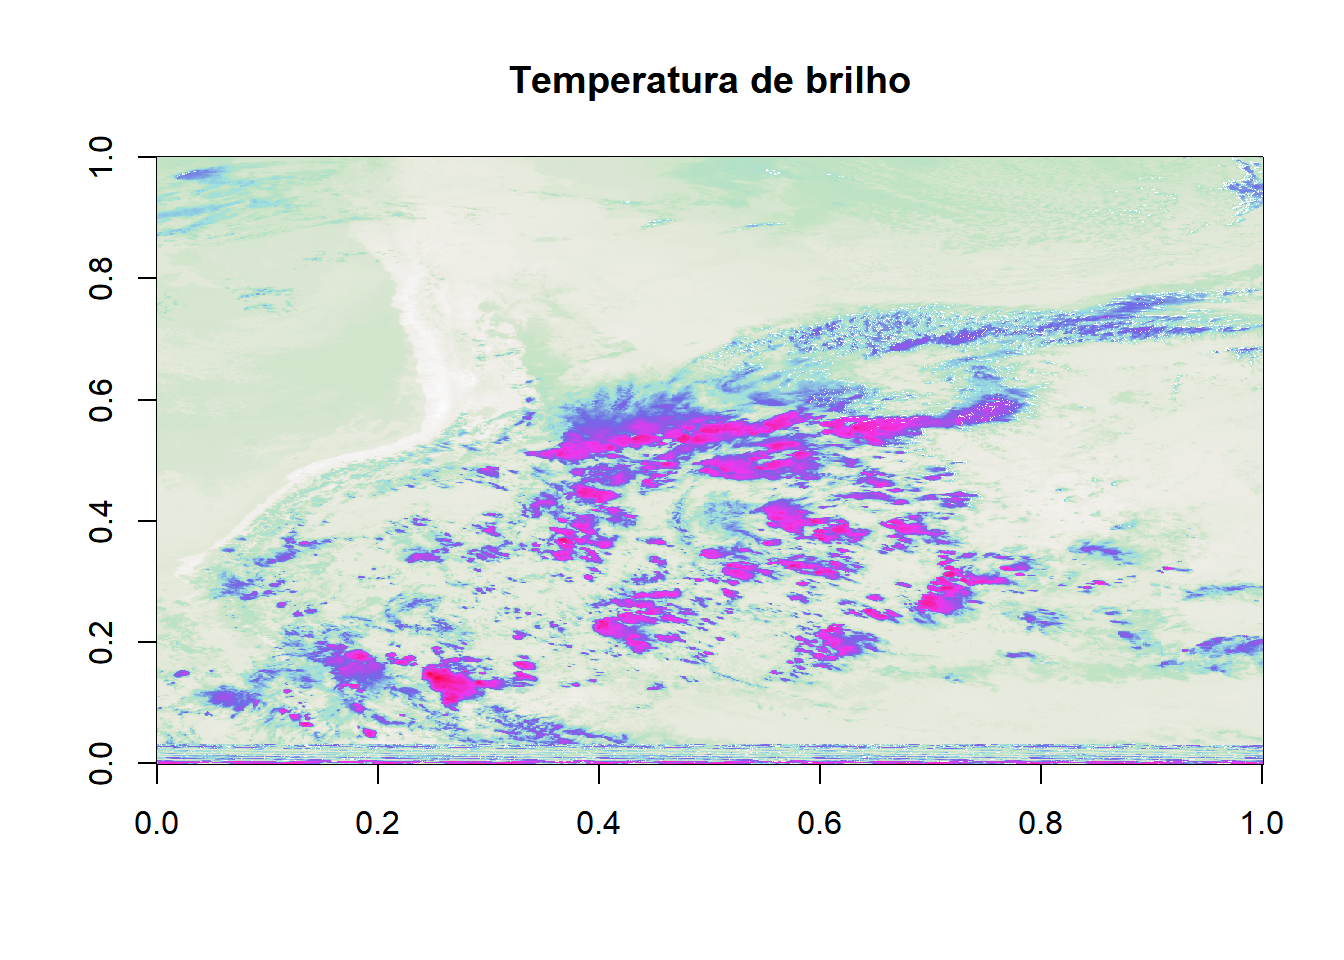
\includegraphics{cursoR_files/figure-latex/unnamed-chunk-80-1.pdf}

Tem algo estranho com esta imagem. O que é? (valendo um sticker).

\begin{Shaded}
\begin{Highlighting}[]
\KeywordTok{library}\NormalTok{(raster, }\DataTypeTok{quietly =} \OtherTok{TRUE}\NormalTok{)}
\NormalTok{l3 <-}\StringTok{ }\KeywordTok{raster}\NormalTok{(}\KeywordTok{t}\NormalTok{(l2[}\DecValTok{1}\OperatorTok{:}\DecValTok{1349}\NormalTok{,}\DecValTok{1}\OperatorTok{:}\DecValTok{1613}\NormalTok{]),}
                     \DataTypeTok{xmn=}\OperatorTok{-}\FloatTok{82.00}\NormalTok{,}
                     \DataTypeTok{ymn=}\OperatorTok{-}\FloatTok{44.96}\NormalTok{,}
                     \DataTypeTok{xmx=}\OperatorTok{-}\FloatTok{82.0}  \OperatorTok{+}\StringTok{ }\NormalTok{(}\FloatTok{0.03593245}\OperatorTok{*}\DecValTok{1349}\NormalTok{), }
                     \DataTypeTok{ymx=}\OperatorTok{-}\FloatTok{44.96} \OperatorTok{+}\StringTok{ }\NormalTok{(}\FloatTok{0.03593245}\OperatorTok{*}\DecValTok{1613}\NormalTok{),}
                     \DataTypeTok{crs =} \KeywordTok{CRS}\NormalTok{(}\StringTok{"+init=epsg:4326"}\NormalTok{))}
\KeywordTok{class}\NormalTok{(l3)}
\end{Highlighting}
\end{Shaded}

\begin{verbatim}
## [1] "RasterLayer"
## attr(,"package")
## [1] "raster"
\end{verbatim}

O capítulo geoespacial será visto no final deste curso. Porém, nesta
etapa vamos usar o pacote \texttt{raster} somente para analisar se os
dados binários foram lidos corretamente.

\begin{Shaded}
\begin{Highlighting}[]
\NormalTok{sp}\OperatorTok{::}\KeywordTok{spplot}\NormalTok{(((l3 }\OperatorTok{+}\StringTok{ }\DecValTok{75}\NormalTok{)}\OperatorTok{/}\DecValTok{100}\NormalTok{)}\OperatorTok{-}\DecValTok{273}\NormalTok{, }\CommentTok{# Estas correções são necessárias. Veja: http://www.cpc.ncep.noaa.gov/products/global_precip/html/README}
           \DataTypeTok{col.regions =} \KeywordTok{cpt}\NormalTok{(}\KeywordTok{find_cpt}\NormalTok{(}\StringTok{"sat"}\NormalTok{)[}\DecValTok{8}\NormalTok{]),}
           \DataTypeTok{at =} \KeywordTok{seq}\NormalTok{(}\OperatorTok{-}\DecValTok{80}\NormalTok{,}\DecValTok{0}\NormalTok{,}\DecValTok{1}\NormalTok{),}
           \DataTypeTok{main =} \StringTok{"Temperatura de brilho (ºC)"}\NormalTok{) }
\end{Highlighting}
\end{Shaded}

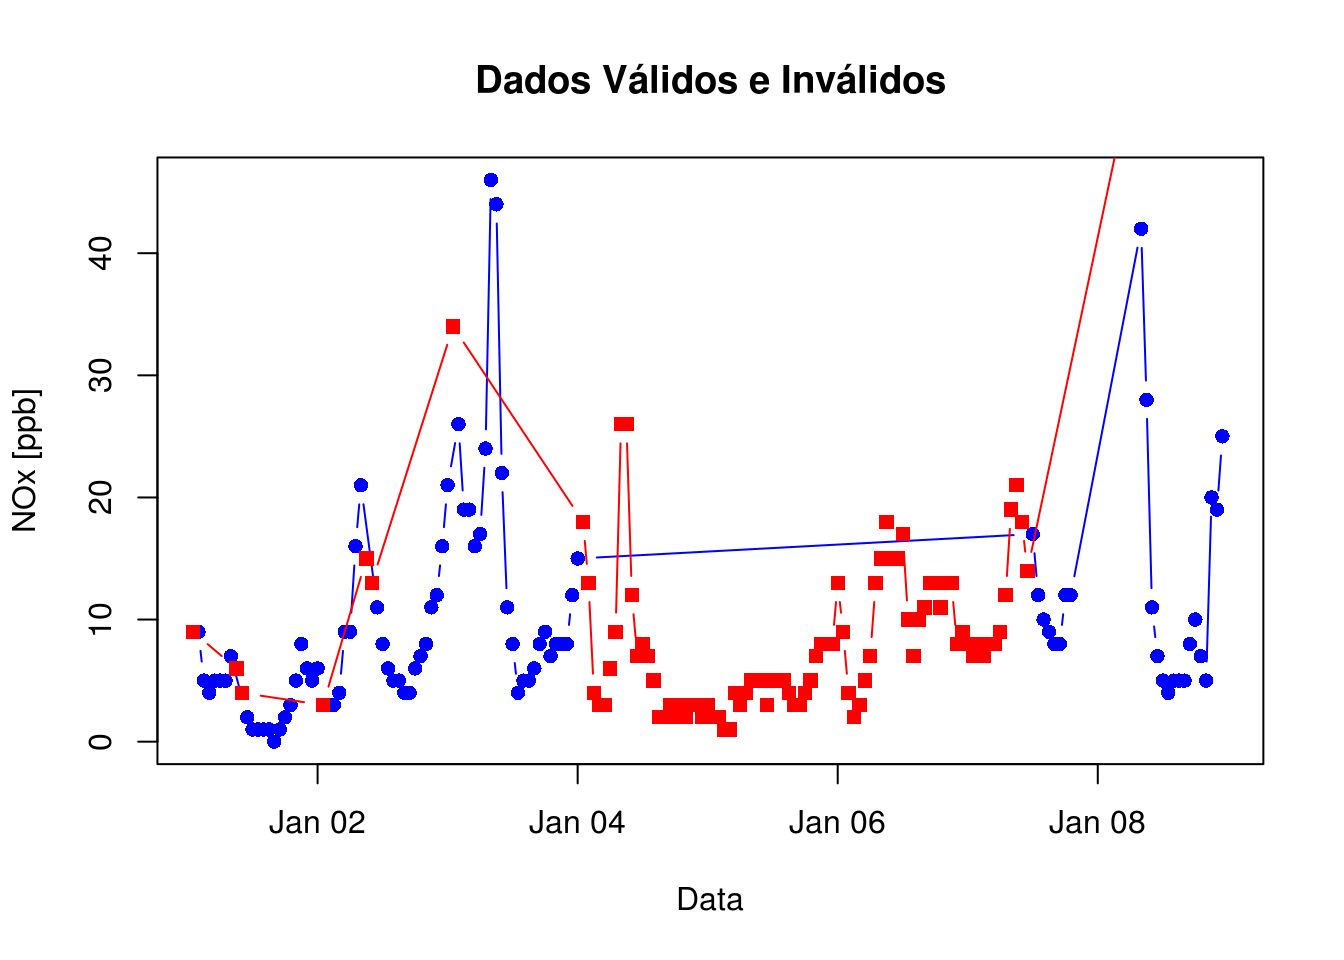
\includegraphics{cursoR_files/figure-latex/unnamed-chunk-82-1.pdf}

\textbf{Escrever dados binários no R}

\chapter{Plotando}\label{plotando}

\section{\texorpdfstring{\texttt{plot}
(base)}{plot (base)}}\label{plot-base}

\textbf{Exemplo}: Dados de qualidade do ar

\begin{Shaded}
\begin{Highlighting}[]
\NormalTok{df <-}\StringTok{ }\KeywordTok{readRDS}\NormalTok{(}\StringTok{"dados/df.rds"}\NormalTok{)}
\KeywordTok{summary}\NormalTok{(df)}
\end{Highlighting}
\end{Shaded}

\begin{verbatim}
##       TipodeRede   TipodeMonitoramento              Tipo     
##  Automático:8581   CETESB:8581         Dados Primários:8581  
##                                                              
##                                                              
##                                                              
##                                                              
##                                                              
##                                                              
##          Data           Hora      CodigoEstação
##  01/01/2014:  24   16:00  : 363   Min.   :95   
##  01/01/2015:  24   12:00  : 361   1st Qu.:95   
##  01/02/2014:  24   14:00  : 361   Median :95   
##  01/04/2014:  24   18:00  : 361   Mean   :95   
##  01/05/2014:  24   13:00  : 360   3rd Qu.:95   
##  01/06/2014:  24   17:00  : 360   Max.   :95   
##  (Other)   :8437   (Other):6415                
##                      NomeEstação                      NomeParâmetro 
##  Cid.Universitária-USP-Ipen:8581   NOx (Óxidos de Nitrogênio):8581  
##                                                                     
##                                                                     
##                                                                     
##                                                                     
##                                                                     
##                                                                     
##  UnidadedeMedida  MediaHoraria    MediaMovel Valido      tempo_char       
##  ppb:8581        Min.   :  0.00   -:8581     Não: 907   Length:8581       
##                  1st Qu.:  9.00              Sim:7674   Class :character  
##                  Median : 18.00                         Mode  :character  
##                  Mean   : 29.87                                           
##                  3rd Qu.: 34.00                                           
##                  Max.   :306.00                                           
##                  NA's   :260                                              
##      tempo                       weekdays             mes           
##  Min.   :2014-01-01 01:00:00   Length:8581        Length:8581       
##  1st Qu.:2014-04-05 14:00:00   Class :character   Class :character  
##  Median :2014-07-05 23:00:00   Mode  :character   Mode  :character  
##  Mean   :2014-07-04 20:22:55                                        
##  3rd Qu.:2014-10-03 10:00:00                                        
##  Max.   :2015-01-02 00:00:00                                        
##                                                                     
##   diajuliano           ano           
##  Length:8581       Length:8581       
##  Class :difftime   Class :character  
##  Mode  :numeric    Mode  :character  
##                                      
##                                      
##                                      
## 
\end{verbatim}

A função \texttt{plot} precisa dos seguintes argumentos:

\begin{Shaded}
\begin{Highlighting}[]
\KeywordTok{args}\NormalTok{(plot)}
\end{Highlighting}
\end{Shaded}

\begin{verbatim}
## function (x, y, ...) 
## NULL
\end{verbatim}

Então, a forma mais fácil de plotar uma variável em função do tempo é:

\begin{Shaded}
\begin{Highlighting}[]
\KeywordTok{plot}\NormalTok{(}\DataTypeTok{x =}\NormalTok{ df}\OperatorTok{$}\NormalTok{tempo, }\DataTypeTok{y =}\NormalTok{ df}\OperatorTok{$}\NormalTok{MediaHoraria)}
\end{Highlighting}
\end{Shaded}

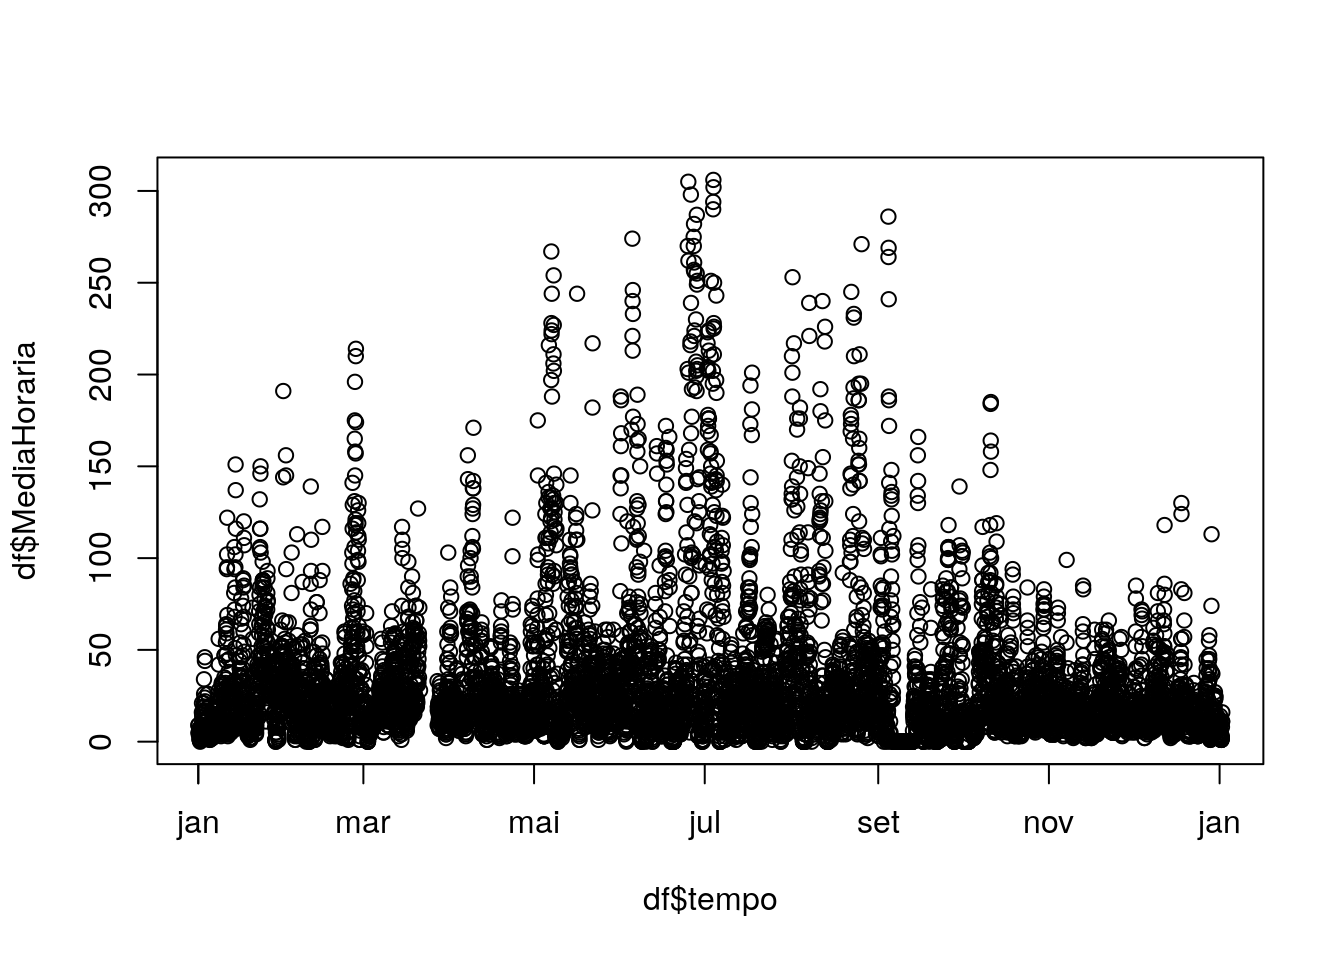
\includegraphics{cursoR_files/figure-latex/unnamed-chunk-85-1.pdf}

Feio, né?\\
Tentando deixar mais bonito\ldots{}

\begin{Shaded}
\begin{Highlighting}[]
\KeywordTok{plot}\NormalTok{(}\DataTypeTok{x =}\NormalTok{ df}\OperatorTok{$}\NormalTok{tempo[}\DecValTok{1}\OperatorTok{:}\DecValTok{100}\NormalTok{], }\DataTypeTok{y =}\NormalTok{ df}\OperatorTok{$}\NormalTok{MediaHoraria[}\DecValTok{1}\OperatorTok{:}\DecValTok{100}\NormalTok{], }\CommentTok{#-- Selecionando uma parte do df!}
     \DataTypeTok{pch =} \DecValTok{16}\NormalTok{, }\CommentTok{#-- Forma do ponto (círculo preenchido)}
     \DataTypeTok{type =} \StringTok{"b"}\NormalTok{, }\CommentTok{#-- Tipo de gráfico ("b" = both, ponto e linha)}
     \DataTypeTok{col =} \StringTok{"blue"}\NormalTok{, }\CommentTok{#-- Cor do elemento (definido pelo type)}
     \DataTypeTok{xlab =} \StringTok{"Data"}\NormalTok{, }\DataTypeTok{ylab =} \StringTok{"NOx [ppb]"}\NormalTok{, }\CommentTok{#-- Nome dos eixos x e y}
     \DataTypeTok{main =} \StringTok{"Gráfico mais Bonito"}\NormalTok{) }\CommentTok{#-- Título do gráfico}
\end{Highlighting}
\end{Shaded}

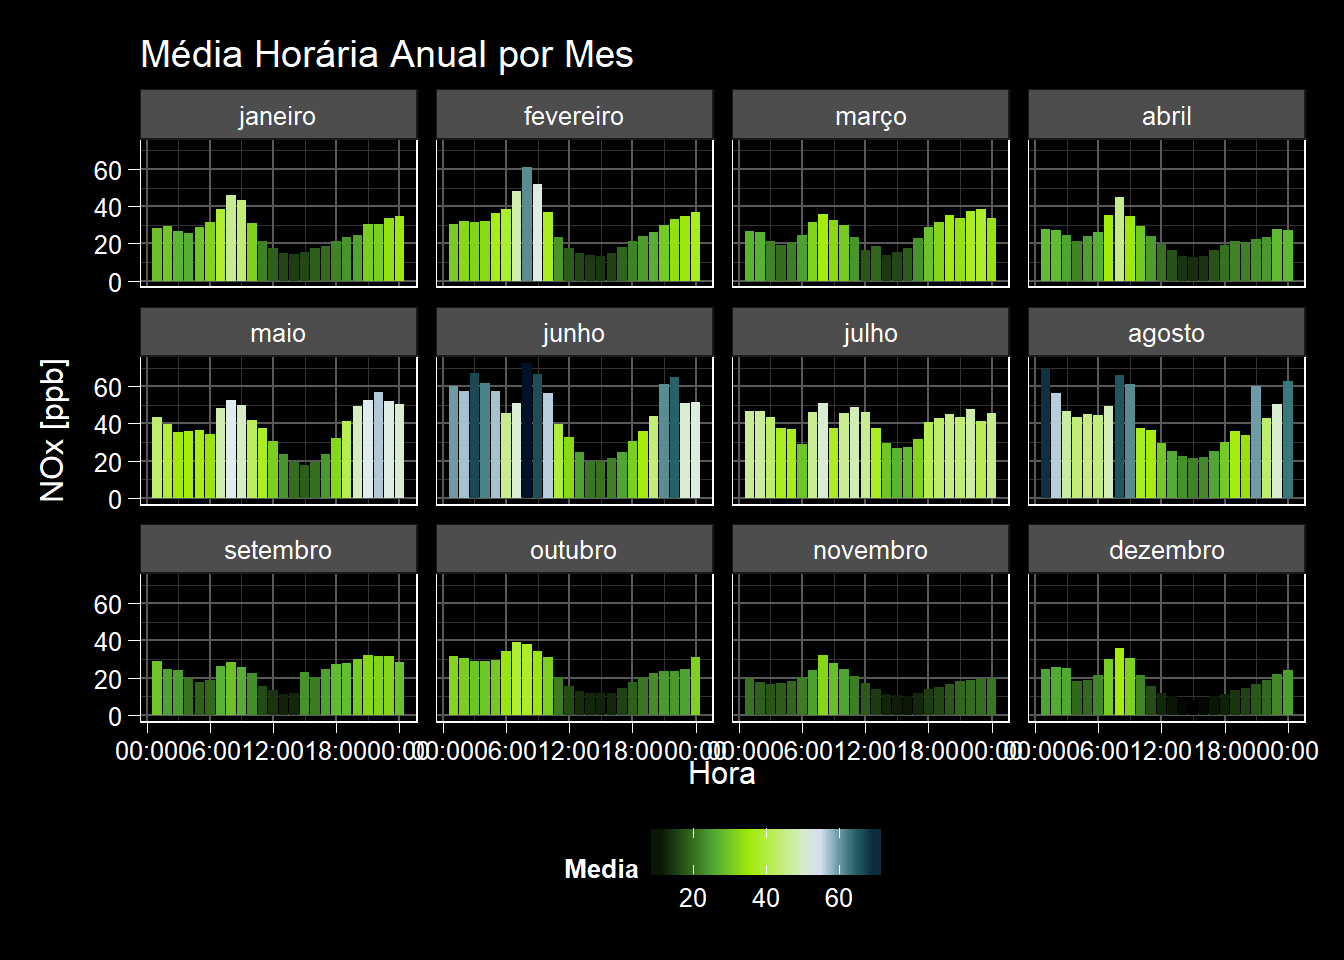
\includegraphics{cursoR_files/figure-latex/unnamed-chunk-86-1.pdf}

Colocando \textbf{DOIS} elementos no mesmo gráfico:

\begin{Shaded}
\begin{Highlighting}[]
\NormalTok{df_parcial <-}\StringTok{ }\NormalTok{df[}\DecValTok{1}\OperatorTok{:}\DecValTok{180}\NormalTok{,] }\CommentTok{#-- Selecionando uma parte do df!}
\KeywordTok{plot}\NormalTok{(}\DataTypeTok{x =}\NormalTok{ df_parcial}\OperatorTok{$}\NormalTok{tempo[df_parcial}\OperatorTok{$}\NormalTok{Valido }\OperatorTok{==}\StringTok{ "Sim"}\NormalTok{], }
     \DataTypeTok{y =}\NormalTok{ df_parcial}\OperatorTok{$}\NormalTok{MediaHoraria[df_parcial}\OperatorTok{$}\NormalTok{Valido }\OperatorTok{==}\StringTok{ "Sim"}\NormalTok{],}
     \DataTypeTok{pch =} \DecValTok{16}\NormalTok{, }\DataTypeTok{type =} \StringTok{"b"}\NormalTok{, }\DataTypeTok{col =} \StringTok{"blue"}\NormalTok{,}
     \DataTypeTok{xlab =} \StringTok{"Data"}\NormalTok{, }\DataTypeTok{ylab =} \StringTok{"NOx [ppb]"}\NormalTok{,}
     \DataTypeTok{main =} \StringTok{"Dados Válidos e Inválidos"}\NormalTok{)}
\KeywordTok{lines}\NormalTok{(}\DataTypeTok{x =}\NormalTok{ df_parcial}\OperatorTok{$}\NormalTok{tempo[df}\OperatorTok{$}\NormalTok{Valido }\OperatorTok{==}\StringTok{ "Não"}\NormalTok{], }
      \DataTypeTok{y =}\NormalTok{ df_parcial}\OperatorTok{$}\NormalTok{MediaHoraria[df}\OperatorTok{$}\NormalTok{Valido }\OperatorTok{==}\StringTok{ "Não"}\NormalTok{], }
      \DataTypeTok{pch =} \DecValTok{15}\NormalTok{, }\DataTypeTok{type =} \StringTok{"b"}\NormalTok{, }\DataTypeTok{col =} \StringTok{"red"}\NormalTok{)}
\end{Highlighting}
\end{Shaded}

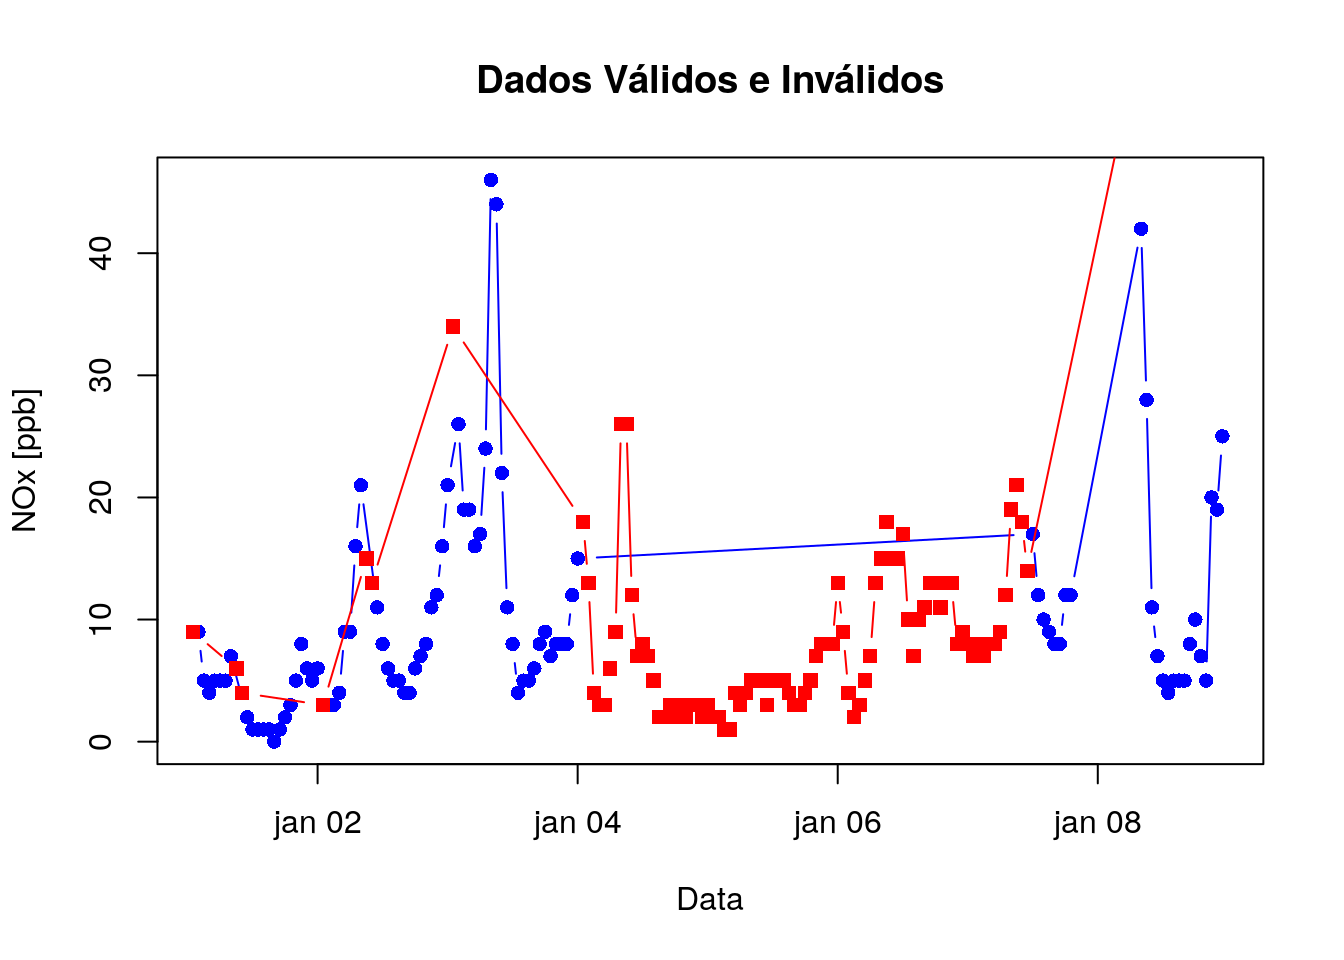
\includegraphics{cursoR_files/figure-latex/unnamed-chunk-87-1.pdf}

\begin{center}\rule{0.5\linewidth}{\linethickness}\end{center}

{\textbf{Desafio}: Coloque uma legenda na figura especificando que os
dados válidos estão em azul e os inválidos em vermelho }

\begin{center}\rule{0.5\linewidth}{\linethickness}\end{center}

A função \texttt{plot} cumpre bem o papel de gerar um gráfico simples, e
até permite algumas customizações, mas ela exige cada vez mais linhas de
código e argumentos dentro das funções para deixar o gráfico ``mais
bonito'' - ao cumprir o desafio, você irá perceber como uma coisa
``simples'' como colocar uma legenda pode exigir muito mais do que
parece!

\section{\texorpdfstring{\texttt{ggplot}
(ggplot2)}{ggplot (ggplot2)}}\label{ggplot-ggplot2}

A função \texttt{ggplot} funciona de um jeito um pouco diferente. Veja a
figura abaixo:

\begin{figure}
\centering
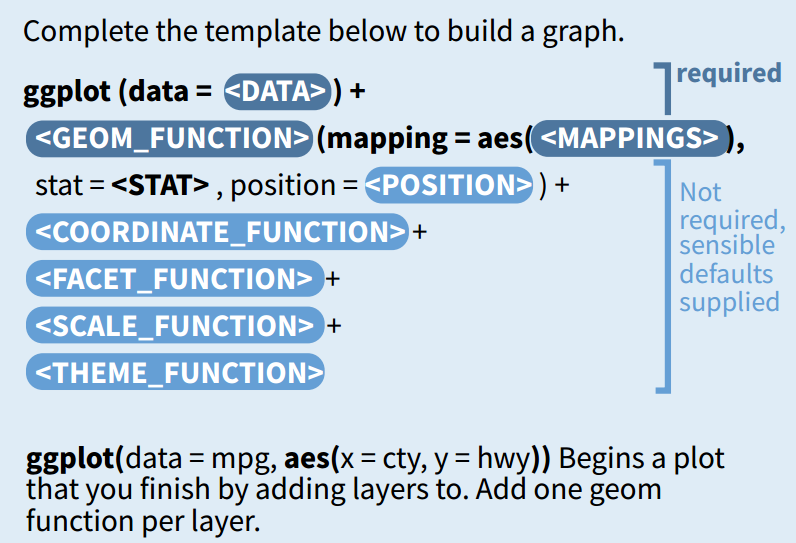
\includegraphics{figuras/ggplot_guide.png}
\caption{Fonte:
\url{https://github.com/rstudio/cheatsheets/raw/master/data-visualization-2.1.pdf}}
\end{figure}

Em vez de uma única função, o gráfico é formado por camadas, sendo que
cada camada é um elemento (\texttt{geom\_...} ou \texttt{stat\_...}) ou
configuração (\texttt{scale\_...\_...}, \texttt{coord\_...},
\texttt{theme} ou \texttt{theme\_...}, \texttt{guides}, \texttt{labs},
etc). Consulte a maioria das opções disponíveis em
\href{https://github.com/rstudio/cheatsheets/raw/master/data-visualization-2.1.pdf}{Data
Visualization Cheatsheet}.

Que tal refazermos os gráficos da seção anterior?

\begin{Shaded}
\begin{Highlighting}[]
\CommentTok{#-- Não esqueça de carregar o pacote!}
\KeywordTok{library}\NormalTok{(ggplot2)}
\end{Highlighting}
\end{Shaded}

\begin{Shaded}
\begin{Highlighting}[]
\KeywordTok{ggplot}\NormalTok{(df, }\KeywordTok{aes}\NormalTok{(}\DataTypeTok{x =}\NormalTok{ tempo, }\DataTypeTok{y =}\NormalTok{ MediaHoraria)) }\OperatorTok{+}
\StringTok{  }\KeywordTok{geom_point}\NormalTok{(}\DataTypeTok{pch =} \DecValTok{1}\NormalTok{)}
\end{Highlighting}
\end{Shaded}

\begin{verbatim}
## Warning: Removed 260 rows containing missing values (geom_point).
\end{verbatim}

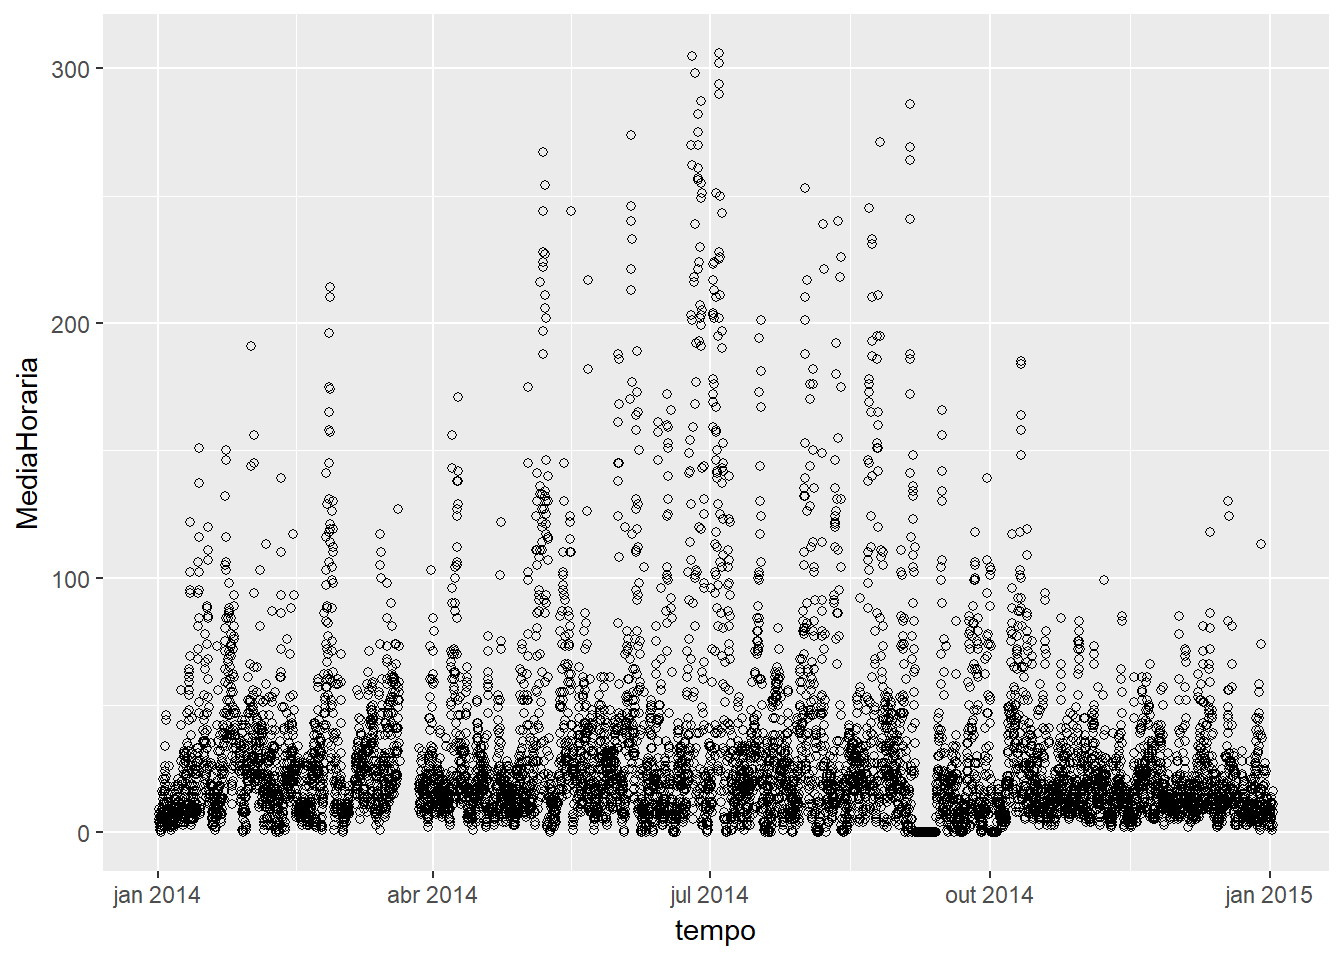
\includegraphics{cursoR_files/figure-latex/unnamed-chunk-89-1.pdf}

\begin{Shaded}
\begin{Highlighting}[]
\KeywordTok{ggplot}\NormalTok{(df[}\DecValTok{1}\OperatorTok{:}\DecValTok{100}\NormalTok{,], }\KeywordTok{aes}\NormalTok{(}\DataTypeTok{x =}\NormalTok{ tempo, }\DataTypeTok{y =}\NormalTok{ MediaHoraria)) }\OperatorTok{+}\StringTok{ }
\StringTok{  }\KeywordTok{geom_line}\NormalTok{(}\DataTypeTok{color =} \StringTok{"blue"}\NormalTok{) }\OperatorTok{+}\StringTok{ }\CommentTok{#-- Linhas...}
\StringTok{  }\KeywordTok{geom_point}\NormalTok{(}\DataTypeTok{color =} \StringTok{"blue"}\NormalTok{, }\DataTypeTok{pch =} \DecValTok{16}\NormalTok{) }\OperatorTok{+}\StringTok{ }\CommentTok{#-- ... com pontos}
\StringTok{  }\KeywordTok{labs}\NormalTok{(}\DataTypeTok{title =} \StringTok{"Gráfico mais Bonito"}\NormalTok{, }\DataTypeTok{x =} \StringTok{"Data"}\NormalTok{, }\DataTypeTok{y =} \StringTok{"NOx [ppb]"}\NormalTok{) }\OperatorTok{+}\StringTok{ }\CommentTok{#-- Títulos}
\StringTok{  }\KeywordTok{theme}\NormalTok{(}\DataTypeTok{plot.title =} \KeywordTok{element_text}\NormalTok{(}\DataTypeTok{hjust =} \FloatTok{0.5}\NormalTok{)) }\CommentTok{#-- Centralizando o título}
\end{Highlighting}
\end{Shaded}

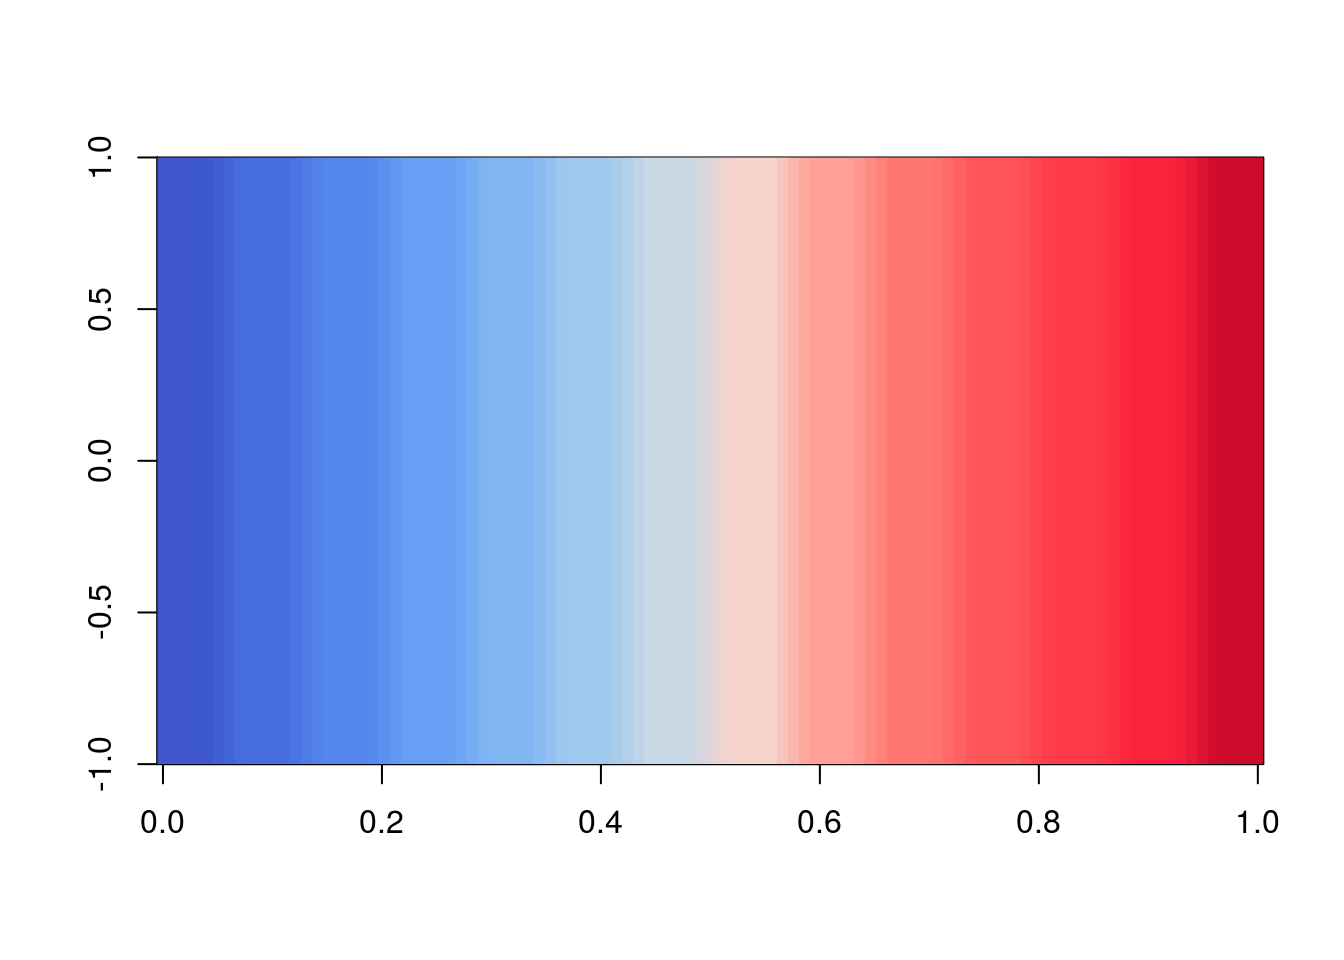
\includegraphics{cursoR_files/figure-latex/unnamed-chunk-90-1.pdf}

Agora o mais interessante:

\begin{Shaded}
\begin{Highlighting}[]
\KeywordTok{ggplot}\NormalTok{(df[}\DecValTok{1}\OperatorTok{:}\DecValTok{180}\NormalTok{,], }\KeywordTok{aes}\NormalTok{(}\DataTypeTok{x =}\NormalTok{ tempo, }\DataTypeTok{y =}\NormalTok{ MediaHoraria)) }\OperatorTok{+}\StringTok{ }
\StringTok{  }\KeywordTok{geom_line}\NormalTok{(}\KeywordTok{aes}\NormalTok{(}\DataTypeTok{color =}\NormalTok{ Valido)) }\OperatorTok{+}
\StringTok{  }\KeywordTok{geom_point}\NormalTok{(}\KeywordTok{aes}\NormalTok{(}\DataTypeTok{color =}\NormalTok{ Valido, }\DataTypeTok{shape =}\NormalTok{ Valido)) }\OperatorTok{+}
\StringTok{  }\KeywordTok{labs}\NormalTok{(}\DataTypeTok{title =} \StringTok{"Dados Válidos e Inválidos"}\NormalTok{, }\DataTypeTok{x =} \StringTok{"Data"}\NormalTok{, }\DataTypeTok{y =} \StringTok{"NOx [ppb]"}\NormalTok{) }\OperatorTok{+}
\StringTok{  }\KeywordTok{scale_color_manual}\NormalTok{(}\DataTypeTok{values =} \KeywordTok{c}\NormalTok{(}\StringTok{"red"}\NormalTok{, }\StringTok{"blue"}\NormalTok{)) }\OperatorTok{+}\StringTok{ }\CommentTok{#-- Definindo as cores manualmente}
\StringTok{  }\KeywordTok{scale_shape_manual}\NormalTok{(}\DataTypeTok{values =} \KeywordTok{c}\NormalTok{(}\DecValTok{15}\NormalTok{, }\DecValTok{16}\NormalTok{)) }\OperatorTok{+}\StringTok{ }\CommentTok{#-- Definindo as formas manualmente}
\StringTok{  }\KeywordTok{theme}\NormalTok{(}\DataTypeTok{plot.title =} \KeywordTok{element_text}\NormalTok{(}\DataTypeTok{hjust =} \FloatTok{0.5}\NormalTok{))}
\end{Highlighting}
\end{Shaded}

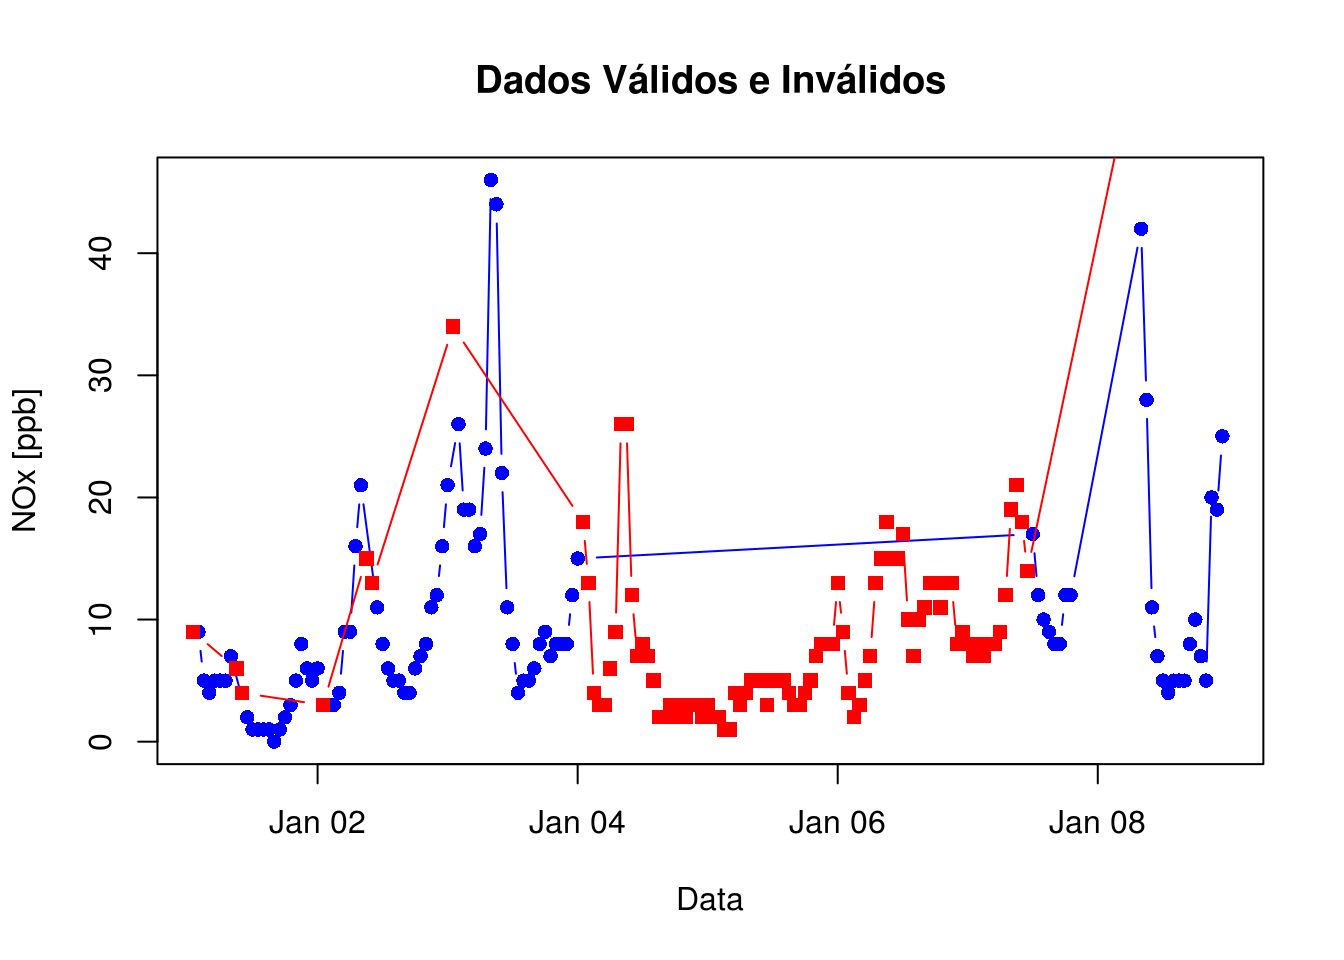
\includegraphics{cursoR_files/figure-latex/unnamed-chunk-91-1.pdf}

{\textbf{Pergunta}: Qual a principal diferença entre o código acima e o
\protect\hyperlink{plot_base}{código usando \texttt{plot}}?}

A função \texttt{ggplot} plota apenas data frames, pois ela mapeia as
variáveis por nomes de colunas. Assim, é preciso
\protect\hyperlink{convert_df}{converter matrizes ou arrays em data
frames}.\\
Uma vantagem de trabalharmos com data frames,
\protect\hyperlink{processing_dfs}{como já vimos antes}, é poder
manipular esses dados de muitas formas possíveis antes de plotá-los.

\textbf{Continuação do Exemplo}: Extraindo algumas informações sobre os
dados

Vamos analisar o ano de 2014:

\begin{itemize}
\tightlist
\item
  \emph{Em média}, como o NOx varia ao longo do dia?

  \begin{itemize}
  \tightlist
  \item
    E para cada dia da semana?\\
  \item
    E para cada mês?
  \end{itemize}
\end{itemize}

Usando algumas funções dentro do pacote \textbf{tidyverse}, que
funcionam bem com o \href{http://r4ds.had.co.nz/pipes.html}{\emph{pipe}
(\texttt{\%\textgreater{}\%})}:

\begin{Shaded}
\begin{Highlighting}[]
\KeywordTok{library}\NormalTok{(tidyverse)}

\NormalTok{df_}\DecValTok{2014}\NormalTok{ <-}\StringTok{ }\KeywordTok{filter}\NormalTok{(df, ano }\OperatorTok{==}\StringTok{ "2014"}\NormalTok{)}
\NormalTok{df_}\DecValTok{2014}\NormalTok{_hour <-}\StringTok{ }\NormalTok{df_}\DecValTok{2014} \OperatorTok\StringTok{ }\CommentTok{#-- A partir do data frame df_2014}
\StringTok{  }\KeywordTok{group_by}\NormalTok{(Hora) }\OperatorTok\StringTok{ }\CommentTok{#-- Agrupe os dados pela coluna hora}
\StringTok{  }\KeywordTok{summarise}\NormalTok{(}\DataTypeTok{Media =} \KeywordTok{mean}\NormalTok{(MediaHoraria, }\DataTypeTok{na.rm =}\NormalTok{ T)) }\OperatorTok\StringTok{ }\CommentTok{#-- E calcule as médias, }
\StringTok{                                                       }\CommentTok{#-- salvando em uma coluna nova}
\StringTok{  }\KeywordTok{mutate}\NormalTok{(}\DataTypeTok{Hora =} \KeywordTok{as.POSIXct}\NormalTok{(}\KeywordTok{strptime}\NormalTok{(Hora, }\StringTok{"%H:%M"}\NormalTok{))) }\OperatorTok\StringTok{ }\CommentTok{#-- Transformando em data}
\StringTok{  }\KeywordTok{ungroup}\NormalTok{() }\CommentTok{#-- Desagrupando}

\KeywordTok{ggplot}\NormalTok{(df_}\DecValTok{2014}\NormalTok{_hour) }\OperatorTok{+}
\StringTok{  }\KeywordTok{scale_x_datetime}\NormalTok{(}\DataTypeTok{date_labels =} \StringTok{"%H:%M"}\NormalTok{) }\OperatorTok{+}\StringTok{ }\CommentTok{#-- Formato de data que aparecerá no eixo x}
\StringTok{  }\KeywordTok{geom_line}\NormalTok{(}\KeywordTok{aes}\NormalTok{(}\DataTypeTok{x =}\NormalTok{ Hora, }\DataTypeTok{y =}\NormalTok{ Media, }\DataTypeTok{group =} \DecValTok{1}\NormalTok{), }\DataTypeTok{color =} \StringTok{"purple"}\NormalTok{) }\OperatorTok{+}
\StringTok{  }\KeywordTok{labs}\NormalTok{(}\DataTypeTok{title =} \StringTok{"Média Horária Anual"}\NormalTok{, }\DataTypeTok{y =} \StringTok{"NOx [ppb]"}\NormalTok{)}
\end{Highlighting}
\end{Shaded}

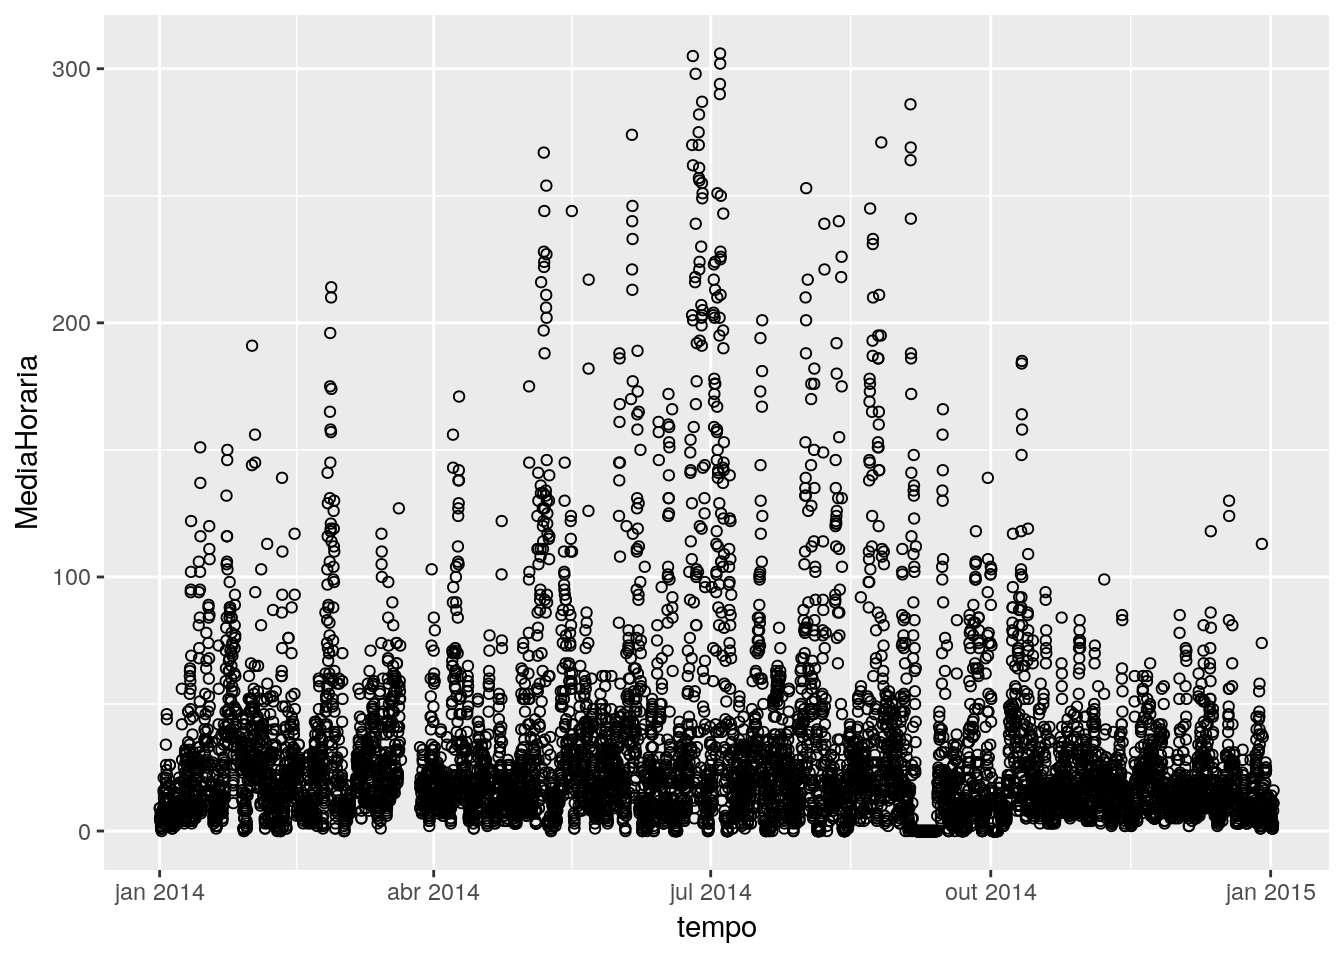
\includegraphics{cursoR_files/figure-latex/unnamed-chunk-92-1.pdf}

\begin{Shaded}
\begin{Highlighting}[]
\NormalTok{df_}\DecValTok{2014}\NormalTok{_weekly <-}\StringTok{ }\NormalTok{df_}\DecValTok{2014} \OperatorTok
\StringTok{  }\KeywordTok{group_by}\NormalTok{(Hora, weekdays) }\OperatorTok\StringTok{ }\CommentTok{#-- Agrupando os dados pelas colunas Hora e weekdays}
\StringTok{  }\KeywordTok{summarise}\NormalTok{(}\DataTypeTok{Media =} \KeywordTok{mean}\NormalTok{(MediaHoraria, }\DataTypeTok{na.rm =}\NormalTok{ T)) }\OperatorTok\StringTok{ }
\StringTok{  }\KeywordTok{ungroup}\NormalTok{() }\OperatorTok\StringTok{ }
\StringTok{  }\KeywordTok{mutate}\NormalTok{(}\DataTypeTok{Hora =} \KeywordTok{as.POSIXct}\NormalTok{(}\KeywordTok{strptime}\NormalTok{(Hora, }\StringTok{"%H:%M"}\NormalTok{))) }\OperatorTok
\StringTok{  }\KeywordTok{mutate}\NormalTok{(}\DataTypeTok{weekdays =} \KeywordTok{factor}\NormalTok{(weekdays, }\DataTypeTok{levels =} \KeywordTok{c}\NormalTok{(}\StringTok{"segunda"}\NormalTok{, }\StringTok{"terça"}\NormalTok{, }\StringTok{"quarta"}\NormalTok{,}
                                                \StringTok{"quinta"}\NormalTok{, }\StringTok{"sexta"}\NormalTok{, }\StringTok{"sábado"}\NormalTok{, }
                                                \StringTok{"domingo"}\NormalTok{))) }\CommentTok{#-- Ordenando os dias da semana}

\KeywordTok{ggplot}\NormalTok{(df_}\DecValTok{2014}\NormalTok{_weekly) }\OperatorTok{+}
\StringTok{  }\KeywordTok{scale_x_datetime}\NormalTok{(}\DataTypeTok{date_labels =} \StringTok{"%H:%M"}\NormalTok{) }\OperatorTok{+}
\StringTok{  }\KeywordTok{geom_col}\NormalTok{(}\KeywordTok{aes}\NormalTok{(}\DataTypeTok{x =}\NormalTok{ Hora, }\DataTypeTok{y =}\NormalTok{ Media), }\DataTypeTok{fill =} \StringTok{"purple"}\NormalTok{) }\OperatorTok{+}
\StringTok{  }\KeywordTok{labs}\NormalTok{(}\DataTypeTok{title =} \StringTok{"Média Horária Anual por Dia da Semana"}\NormalTok{, }\DataTypeTok{y =} \StringTok{"NOx [ppb]"}\NormalTok{) }\OperatorTok{+}
\StringTok{  }\KeywordTok{facet_wrap}\NormalTok{(}\OperatorTok{~}\StringTok{ }\NormalTok{weekdays) }\CommentTok{#-- Criando paineis em função do dia da semana}
\end{Highlighting}
\end{Shaded}

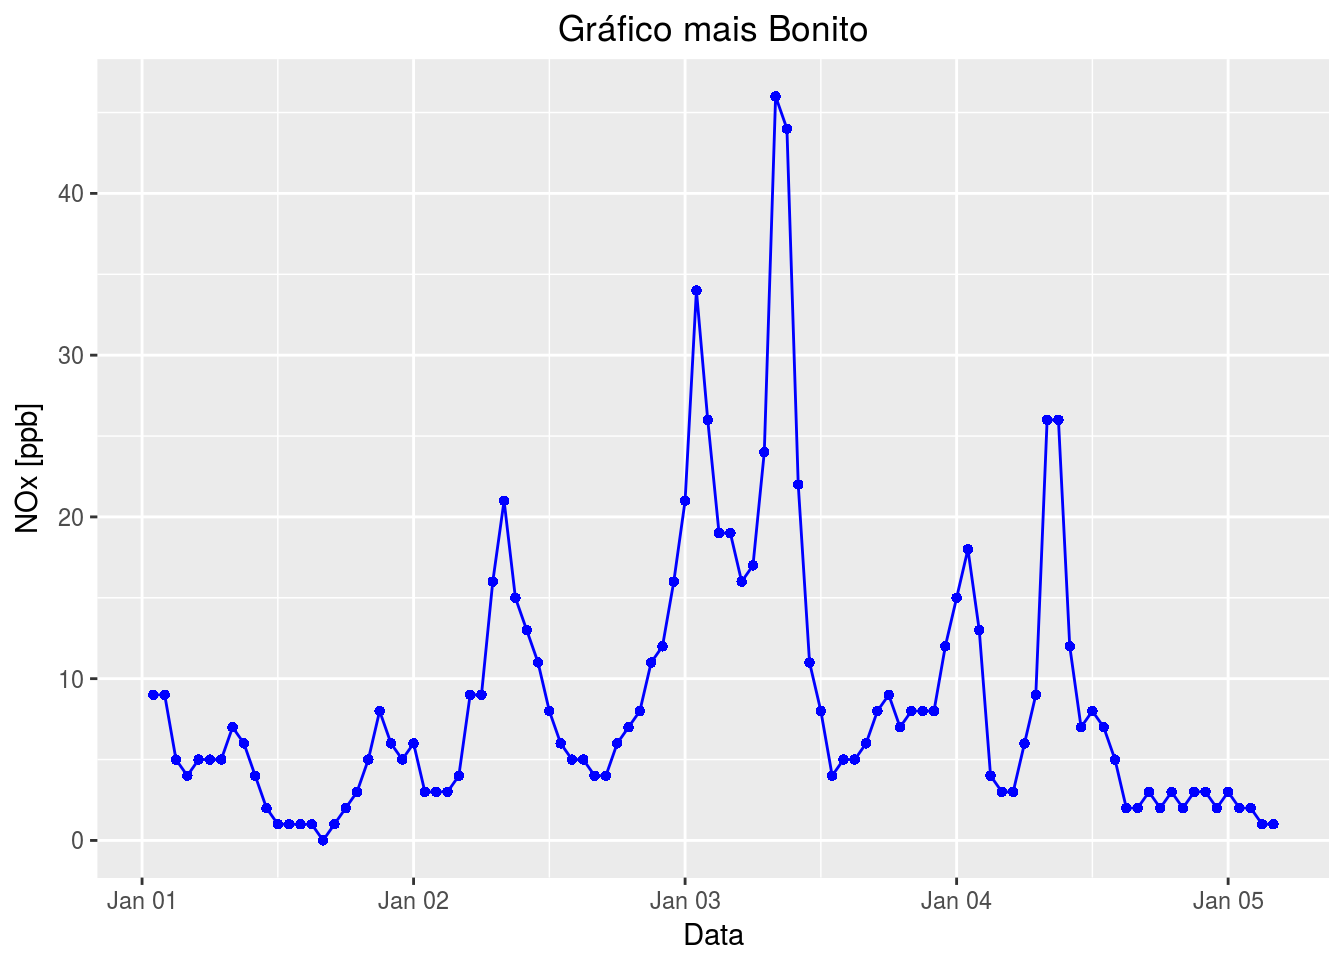
\includegraphics{cursoR_files/figure-latex/unnamed-chunk-93-1.pdf}

\begin{Shaded}
\begin{Highlighting}[]
\NormalTok{df_}\DecValTok{2014}\NormalTok{_monthly <-}\StringTok{ }\NormalTok{df_}\DecValTok{2014} \OperatorTok
\StringTok{  }\KeywordTok{group_by}\NormalTok{(Hora, mes) }\OperatorTok\StringTok{ }\CommentTok{#-- Agrupando os dados pelas colunas Hora e mes}
\StringTok{  }\KeywordTok{summarise}\NormalTok{(}\DataTypeTok{Media =} \KeywordTok{mean}\NormalTok{(MediaHoraria, }\DataTypeTok{na.rm =}\NormalTok{ T)) }\OperatorTok
\StringTok{  }\KeywordTok{ungroup}\NormalTok{() }\OperatorTok
\StringTok{  }\KeywordTok{mutate}\NormalTok{(}\DataTypeTok{Hora =} \KeywordTok{as.POSIXct}\NormalTok{(}\KeywordTok{strptime}\NormalTok{(Hora, }\StringTok{"%H:%M"}\NormalTok{))) }\OperatorTok
\StringTok{  }\KeywordTok{mutate}\NormalTok{(}\DataTypeTok{mes =} \KeywordTok{factor}\NormalTok{(mes, }\DataTypeTok{levels =} \KeywordTok{c}\NormalTok{(}\StringTok{"janeiro"}\NormalTok{, }\StringTok{"fevereiro"}\NormalTok{, }\StringTok{"março"}\NormalTok{, }
                                      \StringTok{"abril"}\NormalTok{, }\StringTok{"maio"}\NormalTok{, }\StringTok{"junho"}\NormalTok{, }\StringTok{"julho"}\NormalTok{,}
                                      \StringTok{"agosto"}\NormalTok{, }\StringTok{"setembro"}\NormalTok{, }\StringTok{"outubro"}\NormalTok{,}
                                      \StringTok{"novembro"}\NormalTok{, }\StringTok{"dezembro"}\NormalTok{))) }\CommentTok{#-- Ordenando os meses}

\KeywordTok{ggplot}\NormalTok{(df_}\DecValTok{2014}\NormalTok{_monthly) }\OperatorTok{+}
\StringTok{  }\KeywordTok{scale_x_datetime}\NormalTok{(}\DataTypeTok{date_labels =} \StringTok{"%H:%M"}\NormalTok{) }\OperatorTok{+}
\StringTok{  }\KeywordTok{geom_col}\NormalTok{(}\KeywordTok{aes}\NormalTok{(}\DataTypeTok{x =}\NormalTok{ Hora, }\DataTypeTok{y =}\NormalTok{ Media), }\DataTypeTok{fill =} \StringTok{"purple"}\NormalTok{) }\OperatorTok{+}
\StringTok{  }\KeywordTok{labs}\NormalTok{(}\DataTypeTok{title =} \StringTok{"Média Horária Anual por Mes"}\NormalTok{, }\DataTypeTok{y =} \StringTok{"NOx [ppb]"}\NormalTok{) }\OperatorTok{+}
\StringTok{  }\KeywordTok{facet_wrap}\NormalTok{(}\OperatorTok{~}\StringTok{ }\NormalTok{mes) }\CommentTok{#-- Criando paineis em função do mês}
\end{Highlighting}
\end{Shaded}

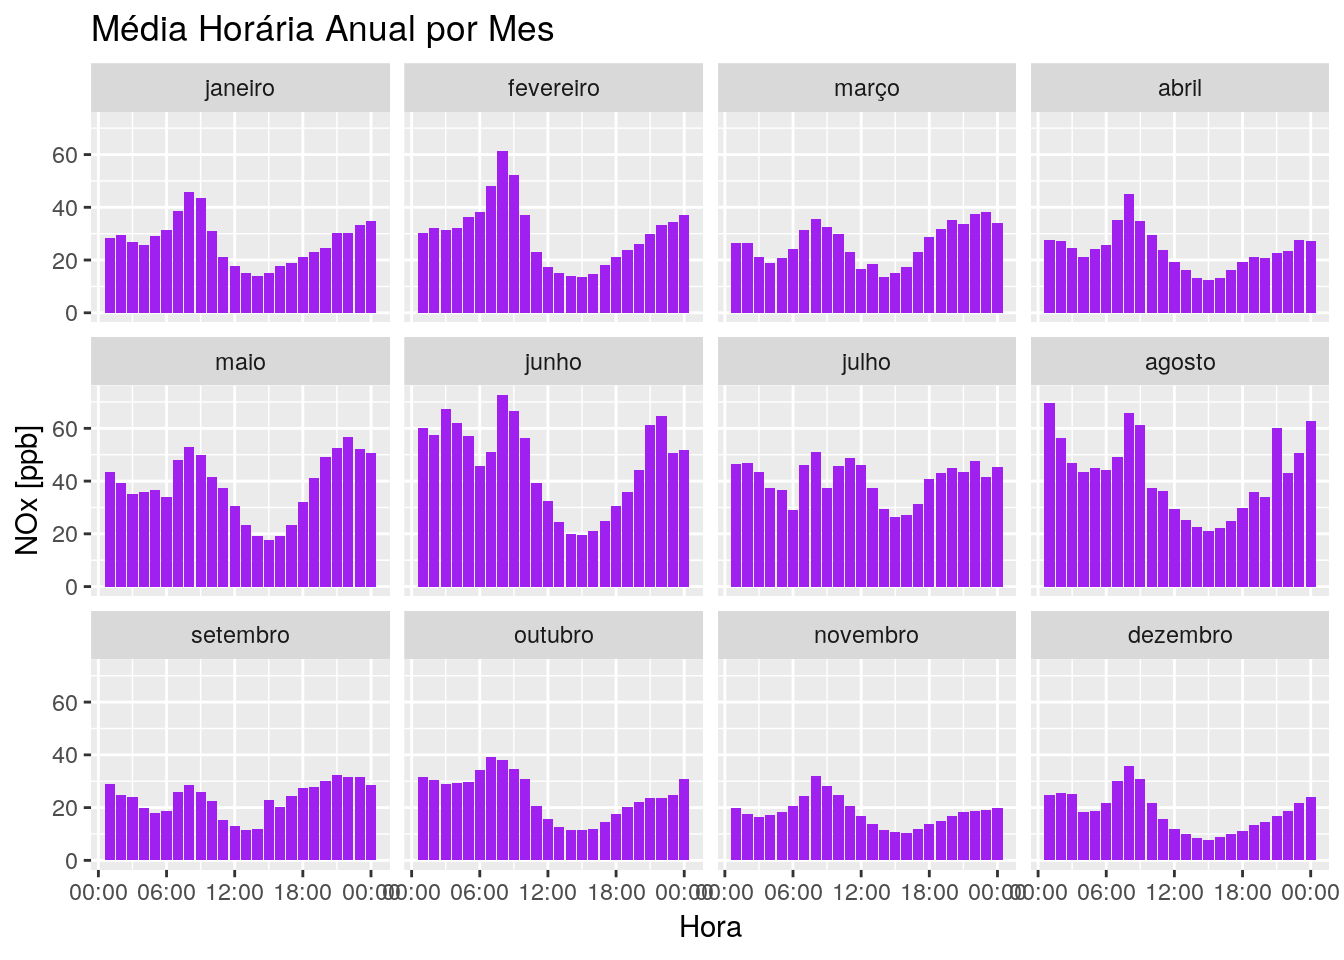
\includegraphics{cursoR_files/figure-latex/unnamed-chunk-94-1.pdf}

\begin{center}\rule{0.5\linewidth}{\linethickness}\end{center}

{\textbf{Exercício}: \emph{Em média}, como \textbf{os dados válidos} de
NOx variam mensalmente ao longo do ano de 2014? Faça um gráfico.}

{\textbf{Desafio}: Ainda é possível melhorar os gráficos acima! Pesquise
como:}

{* Diminuir a quantidade de horários no eixo x}\\
{* Separar por dias da semana e meses a partir da coluna ``tempo'', não
precisando usar as colunas de caracteres e consequentemente ordená-las
manualmente}

\begin{center}\rule{0.5\linewidth}{\linethickness}\end{center}

\subsection{Explorando outras escalas de cores e
temas}\label{explorando-outras-escalas-de-cores-e-temas}

Pacotes \textbf{veinreport} e \textbf{cptcity}

\begin{Shaded}
\begin{Highlighting}[]
\NormalTok{devtools}\OperatorTok{::}\KeywordTok{install_github}\NormalTok{(}\StringTok{"atmoschem/veinreport"}\NormalTok{)}
\end{Highlighting}
\end{Shaded}

\begin{Shaded}
\begin{Highlighting}[]
\KeywordTok{library}\NormalTok{(veinreport)}
\KeywordTok{library}\NormalTok{(cptcity)}
\end{Highlighting}
\end{Shaded}

Refazendo alguns gráficos:

\begin{Shaded}
\begin{Highlighting}[]
\KeywordTok{ggplot}\NormalTok{(df, }\KeywordTok{aes}\NormalTok{(}\DataTypeTok{x =}\NormalTok{ tempo, }\DataTypeTok{y =}\NormalTok{ MediaHoraria)) }\OperatorTok{+}\StringTok{ }
\StringTok{  }\KeywordTok{geom_line}\NormalTok{(}\KeywordTok{aes}\NormalTok{(}\DataTypeTok{color =}\NormalTok{ MediaHoraria)) }\OperatorTok{+}
\StringTok{  }\KeywordTok{labs}\NormalTok{(}\DataTypeTok{x =} \StringTok{"Data"}\NormalTok{, }\DataTypeTok{y =} \StringTok{"NOx [ppb]"}\NormalTok{) }\OperatorTok{+}
\StringTok{  }\KeywordTok{scale_color_gradientn}\NormalTok{(}\DataTypeTok{colours =} \KeywordTok{cpt}\NormalTok{()) }\OperatorTok{+}\StringTok{ }\CommentTok{#-- Definindo as cores com uma escala gradiente}
\StringTok{  }\KeywordTok{theme_black}\NormalTok{()}
\end{Highlighting}
\end{Shaded}

\begin{verbatim}
## Warning: Removed 1 rows containing missing values (geom_path).
\end{verbatim}

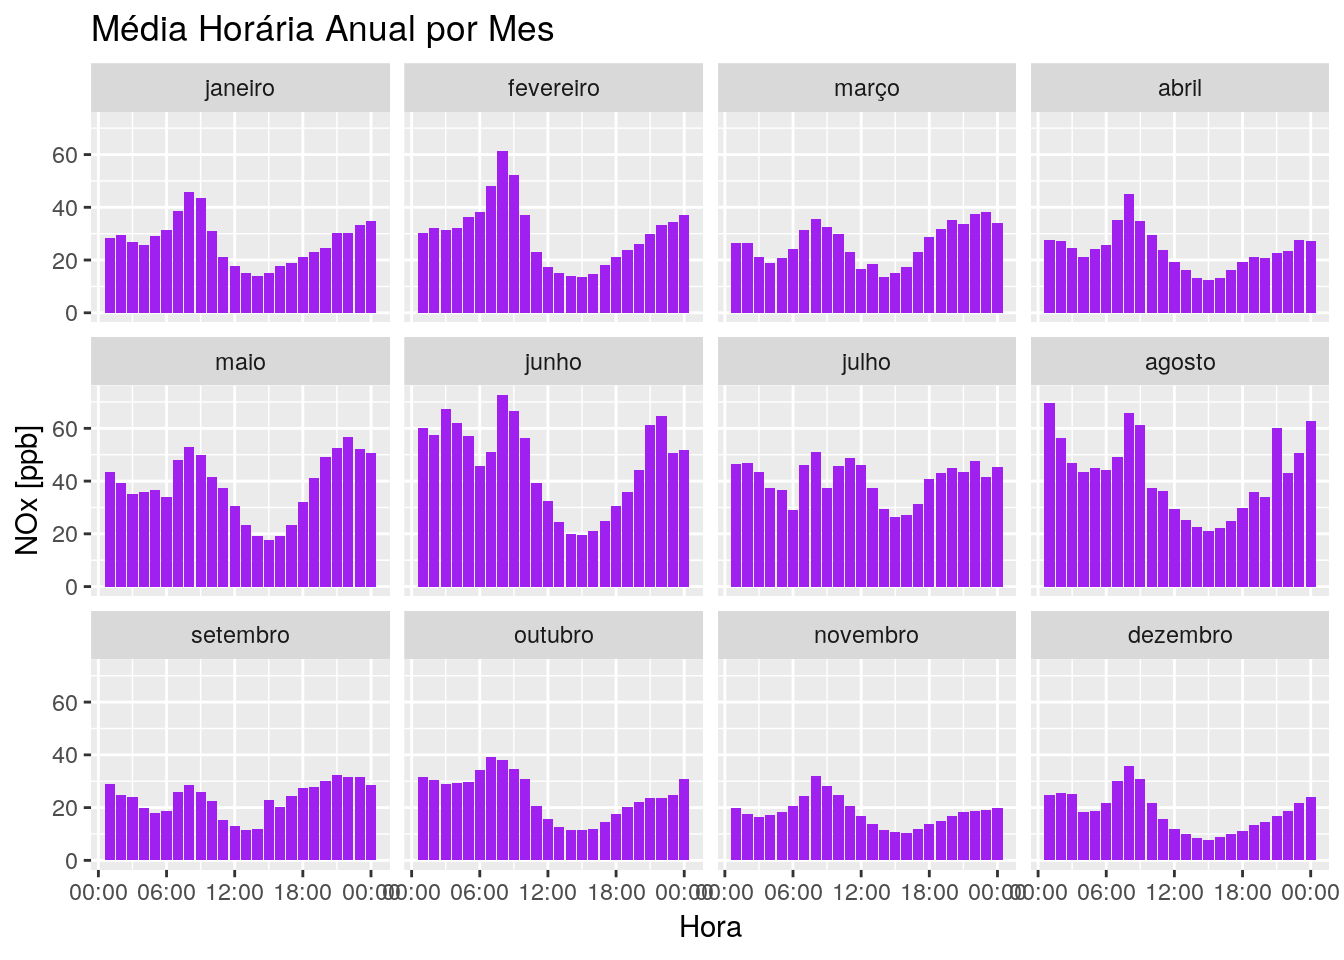
\includegraphics{cursoR_files/figure-latex/unnamed-chunk-97-1.pdf}

Experimentando escalas de cores com a função \texttt{lucky}:

\begin{Shaded}
\begin{Highlighting}[]
\KeywordTok{ggplot}\NormalTok{(df_}\DecValTok{2014}\NormalTok{_monthly) }\OperatorTok{+}
\StringTok{  }\KeywordTok{scale_x_datetime}\NormalTok{(}\DataTypeTok{date_labels =} \StringTok{"%H:%M"}\NormalTok{) }\OperatorTok{+}
\StringTok{  }\KeywordTok{geom_col}\NormalTok{(}\KeywordTok{aes}\NormalTok{(}\DataTypeTok{x =}\NormalTok{ Hora, }\DataTypeTok{y =}\NormalTok{ Media, }\DataTypeTok{fill =}\NormalTok{ Media)) }\OperatorTok{+}
\StringTok{  }\KeywordTok{labs}\NormalTok{(}\DataTypeTok{title =} \StringTok{"Média Horária Anual por Mes"}\NormalTok{, }\DataTypeTok{y =} \StringTok{"NOx [ppb]"}\NormalTok{) }\OperatorTok{+}
\StringTok{  }\KeywordTok{scale_fill_gradientn}\NormalTok{(}\DataTypeTok{colors =} \KeywordTok{lucky}\NormalTok{()) }\OperatorTok{+}\StringTok{ }\CommentTok{#-- Definindo as cores com uma escala gradiente aleatória}
\StringTok{  }\KeywordTok{theme_black}\NormalTok{() }\OperatorTok{+}
\StringTok{  }\KeywordTok{theme}\NormalTok{(}\DataTypeTok{legend.position =} \StringTok{"bottom"}\NormalTok{, }\DataTypeTok{legend.direction =} \StringTok{"horizontal"}\NormalTok{) }\OperatorTok{+}\StringTok{ }\CommentTok{#-- Colocando a legenda na parte de baixo da figura}
\StringTok{  }\KeywordTok{facet_wrap}\NormalTok{(}\OperatorTok{~}\StringTok{ }\NormalTok{mes) }\CommentTok{#-- Criando paineis em função do mês}
\end{Highlighting}
\end{Shaded}

\begin{verbatim}
## Colour gradient: nd_basic_Cyan_White_Magenta, number: 5225
\end{verbatim}

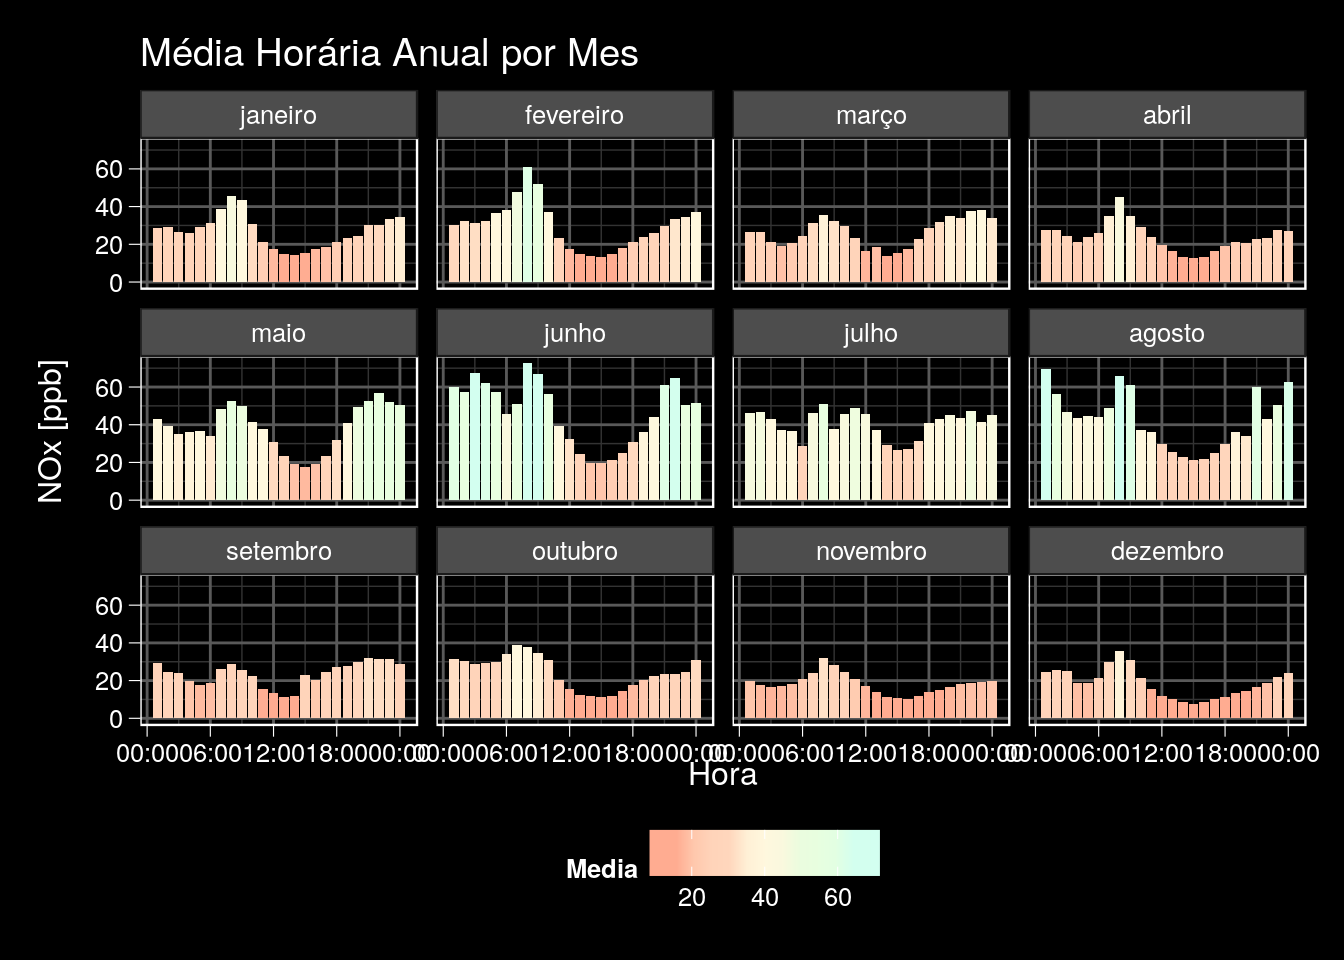
\includegraphics{cursoR_files/figure-latex/unnamed-chunk-98-1.pdf}

\textbf{Este é só o começo!}
\href{http://r-statistics.co/Top50-Ggplot2-Visualizations-MasterList-R-Code.html}{Veja
aqui um pouco mais das muitas aplicações do \texttt{ggplot}}.

\chapter{Estruturas de Controle}\label{loop}

\section{if-else}\label{if-else}

\section{for}\label{for}

\section{while}\label{while}

\section{repeat}\label{repeat}

\section{lapply}\label{lapply}

\section{sapply}\label{sapply}

\section{split}\label{split}

\section{tapply}\label{tapply}

\section{apply}\label{apply}

\section{mapply}\label{mapply}

\chapter{De Scripts a Funções e de Funções a Pacotes}\label{fx}

Em breve.

\chapter{\texorpdfstring{Geo Spatial: \texttt{raster}, \texttt{sf} e
\texttt{stars}}{Geo Spatial: raster, sf e stars}}\label{geo}

Em breve.

\begin{itemize}
\tightlist
\item
  \href{https://leanpub.com/rprogramming}{R Programming for Data Science
  (Leanpub)}\\
\item
  \href{http://www.cookbook-r.com/Graphs/}{R Graphics Cookbook (Cookbook
  for R)}\\
\item
  \href{https://cran.r-project.org/doc/manuals/r-release/R-intro.html}{An
  Introduction to R (CRAN)}\\
\item
  \href{https://cran.r-project.org/doc/manuals/r-release/R-data.html}{R
  Data Import/Export (CRAN)}\\
\item
  \href{https://www.rstudio.com/resources/cheatsheets/}{RStudio Cheat
  Sheets (RStudio)}\\
\item
  \href{https://www.rstudio.com/resources/webinars/}{Webinars and Videos
  On Demand (RStudio)}\\
\item
  \href{https://www.rstudio.com/online-learning/}{Online Learning
  (RStudio)}\\
\item
  \href{https://www.tidyverse.org/learn/}{Learn the tidyverse
  (Tidyverse)}
\item
  \href{https://cran.r-project.org/doc/manuals/r-release/R-exts.html}{Writing
  R Extensions (CRAN)}\\
\item
  \href{https://cran.r-project.org/doc/manuals/r-release/R-ints.html}{R
  Internals (CRAN)}\\
\item
  \href{https://cran.r-project.org/doc/manuals/r-release/R-lang.html}{R
  Language Definition (CRAN)}
\end{itemize}

\begin{center}\rule{0.5\linewidth}{\linethickness}\end{center}

\emph{Quer fazer um documento com o mesmo estilo do nosso? Leia}
\href{https://bookdown.org/yihui/bookdown/}{bookdown: Authoring Books
and Technical Documents with R Markdown (bookdown.org)}

\bibliography{book.bib,packages.bib}


\end{document}
